
\documentclass[a4paper]{report}
% scopiazzato dal template di Matteo Longeri (grazie!)
%%%%%%%%%%%%%%%%%%%%%%%%%%%%%%%%%%%%%%%%%%%%%%%%%%%%%%
% o article, book, ...



%%%%%%%%%%%%%%%%%%%%%%%%%%%%%%%%%%%%%%%%%%%%%%%%%%%%%%
% packages...
\usepackage[utf8]{inputenc}
\usepackage[english,italian]{babel}
\usepackage[hyphens]{url}

\usepackage{todonotes}

% Per generare il file PDF aderente alle specifiche PDF/A-1b. Verificarne poi la validità.
%\usepackage[a-1b]{pdfx}

\usepackage{hyperref}
\usepackage{graphicx}


%%%%%%%%%%%%%%%%%%%%%%%%%%%%%%%%%%%%%%%%%%%%%%%%%%%%%
\begin{document}

% Frontespizio
\begin{titlepage}
\begin{center}

\includegraphics[width=\textwidth]{Logo.jpg}\\
{\large{\bf Corso di Laurea Triennale in Informatica}}
\end{center}
\vspace{12mm}
\begin{center}
{\huge{\bf Studio sull'incidentalit\'a stradale}}\\
\vspace{4mm}
{\huge{\bf tramite dataset aperti}}\\
\end{center}
\vspace{12mm}
\begin{flushright}
{\large{\bf Tesi di Laurea di:}}\\
{\large{\bf Gabriele Padovani}}\\
{\large{\bf Matr. 909165}}\\
\end{flushright}
\vspace{4mm}
\begin{flushleft}
{\large{\bf Relatore:}}\\
{\large{\bf Andrea Trentini}}\\
\vspace{4mm}
{\large{\bf Correlatore:}}\\
{\large{\bf CORREL}}\\
\end{flushleft}
\vspace{12mm}
\begin{center}
{\large{\bf Anno Accademico 2020/2021}}
\end{center}
\end{titlepage}


\tableofcontents

\listoftodos

%%%%%%%%%%%%%%%%%%%%%%%%%%%%%%%%%%%%%%%%%%%%%%%%%%%%%%
\chapter{Introduzione}

%%%%%%%%%%%%%%%%%%%%%%%%%%%%%%%%%%%%%%%%%%%%%%%%%%%%%%
\section{Origine dei dati}

\subsection{Dati riguardanti incidenti}
La maggior parte dei dati utilizzati in questo lavoro provengono 
dall'Istituto nazionale di statistica, 
in particolare dall'archivio di dati non geolocalizzati su incidenti stradali in Italia.
Questo dataset contiene un'ampia gamma di campi, tra cui ora, 
mese, giorno della settimana in cui è avvenuto l'incidente, 
ma anche dati sui passeggeri, la natura dell'incidente e il tipo di strada. 
Particolarmente interessanti sono anche i campi riguardanti il tipo di incrocio a cui è 
avvenuto il sinistro, come rettilineo, rotonda o semaforo.

\todo{Metto i link per citare fonti online?}
Per quanto riguarda i dati geolocalizzati, la fonte è invece il sito web TheSubmarine, %(https://thesubmarine.it/)
che in un articolo riguardante l'incidentalità a Milano, 
ha ottenuto dall'ente Istat la pubblicazione di una parte degli 
incidenti avvenuti nella città nel 2016, con la relativa posizione.
Il dataset in questione è abbastanza povero, e contiene solamente l'incidente con la 
propria posizione, indicata tramite coordinate geografiche.

\todo{Migliorare, ho chiesto sulla sezione servizi del sito}
L'ultimo dataset, trovato dopo veloce cosultazione con un dipendente Istat, è stato 
il dataset ACI.
\'E stato consigliato in quanto, questi dati, specifici a autostrade e strade statali, 
indicano anche il nome della rispettiva via.

\subsection{Dati riguardanti autovelox}
Un primo dataset individuato, che riguardasse delle posizioni degli autovelox fissi, 
è stato una mappa GoogleMyMaps creata da un utente anonimo, 
dunque senza un modo di provare l'autenticità dei dati.

Il dataset utilizzato, invece, è stato ottenuto tramite OpenStreetMaps, ricavando solo gli autovelox 
in Milano. 
Per restringere il campo di ricerca a solo Milano, si è fatto uso delle Overpass API, specifiche per 
OpenStreetMaps, eseguendo la seguente query: 

\todo{Package per visualizzare codice?}
[out:json];\\
node({{bbox}})["highway"="speed\_camera"];\\
out meta;

Il dataset ricavato non permette di capire quando gli autovelox siano stati installati.
% Non è una fonte molto sicura
Tuttavia il sito web ztlmilano contiene un articolo nel quale specifica una lista di 
autovelox installati nel 2014, considerando che il dataset di OpenStreetMaps è aggiornato, 
è possibile ricavare la posizione precisa di questi ultimi.
\todo{Codice utilizzato per autovelox\_2014.csv}

\subsection{Dati riguardanti il meteo}
\todo{non so ancora se usarli}

\subsection{Dati riguardanti trasporti pubblici}
I dati riguardanti i trasporti pubblici trovati hanno due provenienze, i primi sono 
dati riferiti alle linee ATM, scaricati sul sito del comune di milano.
Dallo stesso sito proviene anche il dataset riguardante gli autobus turistici, che 
contiene in particolare le aree di sosta di questi ultimi.

\subsection{Dati riguardanti piste ciclabili}
Oltre al sito principale del comune di Milano, esiste un secondo sito web dedicato 
unicamente ai dati geolocalizzati. Su questo sito è disponibile un dataset contenente 
i percorsi delle piste ciclabili di Milano.

\subsection{Dati riguardanti autostrade e manto stradale}
\todo{devo guardare il dataset del manto stradale che ho trovato}

%%%%%%%%%%%%%%%%%%%%%%%%%%%%%%%%%%%%%%%%%%%%%%%%%%%%%%
\section{Scopo del lavoro}

%%%%%%%%%%%%%%%%%%%%%%%%%%%%%%%%%%%%%%%%%%%%%%%%%%%%%%
\section{Dati mancanti}

\subsection{Dati riguardanti pavè}
\todo{cercare dati su manto stradale}

\subsection{Dati riguardanti traffico stradale}
\todo{devo ancora cercare se c'è un dataset sul traffico}


%%%%%%%%%%%%%%%%%%%%%%%%%%%%%%%%%%%%%%%%%%%%%%%%%%%%%%
\chapter{Dati Geolocalizzati}

\section{Incidenti}

Controllando i dati trovati, in particolare come questi siano distributi, 
si nota subito che gli incidenti a Milano sono per buona parte uniformemente sparsi in tutta la città, 
con più alta concentrazione in alcuni punti di interesse, come Piazzale Loreto, Zona Navigli 
e Monumentale, e Corso Ventidue Marzo.

\begin{figure}
    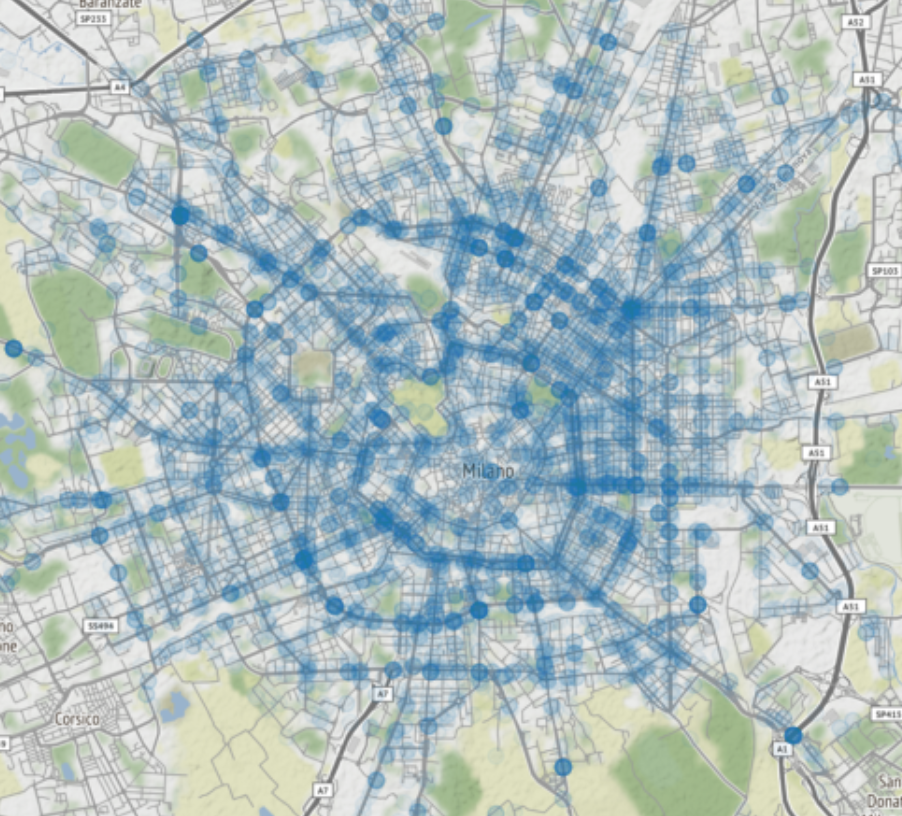
\includegraphics[width=\linewidth]{../src/incidenti/geo_incidenti.png}
    \caption{Distribuzione di incidenti a Milano}
    \label{fig:geo_incidenti}
\end{figure}
%\ref{fig:geo_incidenti}


%...


%\clearpage
\section{Incidenti e Linee dei Trasporti Pubblici}

Il dataset dei tragitti dei trasporti pubblici copre molta più superficie rispetto a 
quello degli incidenti.
Dopo aver eliminato alcune linee di autobus che risultavano troppo in periferia, 
si nota comunque che i trasporti pubblici coprono la maggior parte di Milano.

\begin{figure}
    \includegraphics[width=\linewidth]{../src/atm/mappa_2.png}
    \caption{Linee Autobus e Tram a Milano}
    \label{fig:geo_trasporti}
\end{figure}
%\ref{fig:geo_trasporti}


Se a questi ultimi vengono sovrapposti i dati sugli incidenti, 
si pu\'o notare che la maggior parte dei luoghi con alta concentrazione di incidenti sono 
attraversati da linee di autobus. Nel caso di Corso Ventidue Marzo, si ha anche una linea di tram.


%...


Dalla sovrapposizione delle mappe, si pu\'o notare anche che, alcune strade con alta incidentalit\'a 
sono parallele a linee di autobus. Un esempio è quello di zona Navigli, 
dove le vie interessate sono:
Viale Gian Galeazzo e Viale Beatrice D'Este, parallele a Viale Col di Lana e Viale Bligny.
La stessa cosa si pu\'o notare su Viale Gabriele D'Annunzio e Viale Gorizia e Coni Zugna.

\begin{figure}
    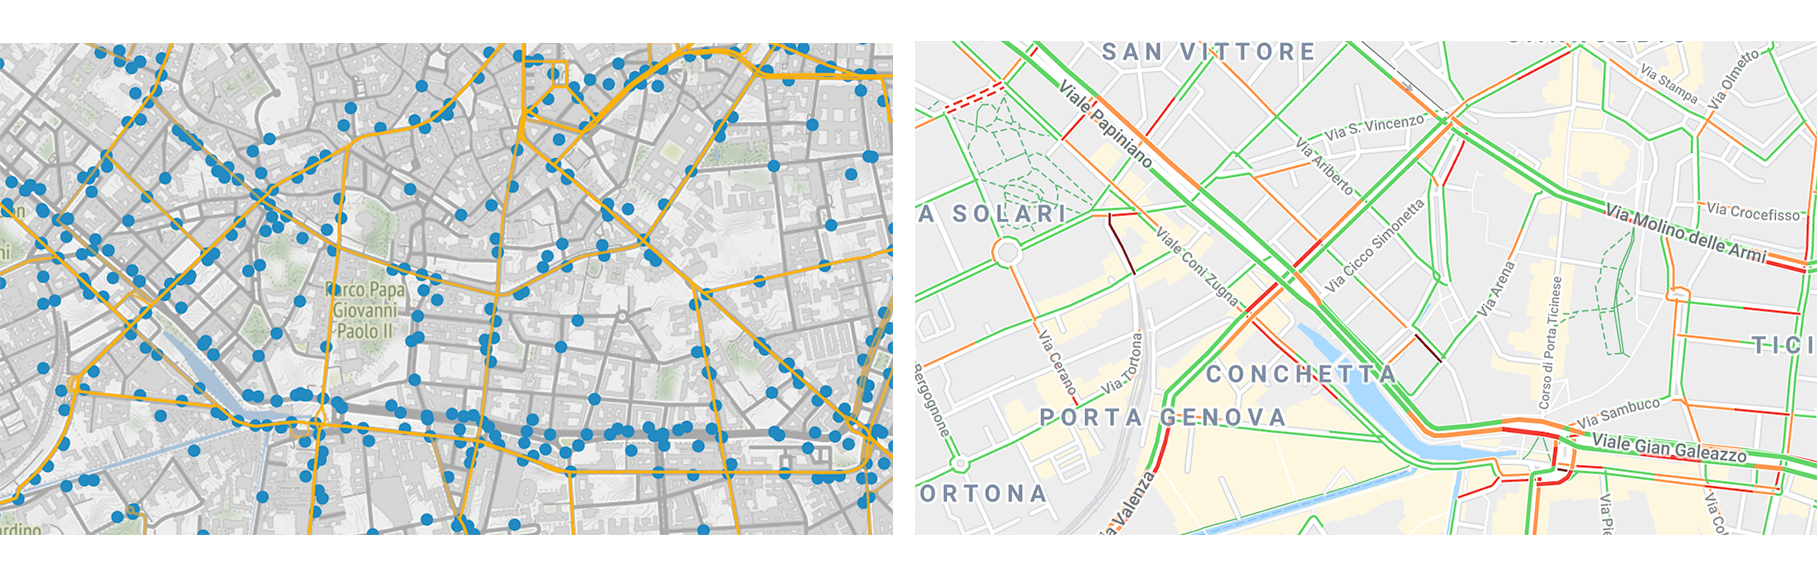
\includegraphics[width=\linewidth]{../src/atm/navigli.png}
    \caption{Linee Autobus e Tram a Milano}
    \label{fig:navigli}
\end{figure}
%\ref{fig:navigli}


Anche vicino a corso Ventidue Marzo si pu\'o notare lo stesso fenomeno, 
tra Viale Bianca Maria e Viale Premuda.

\begin{figure}
    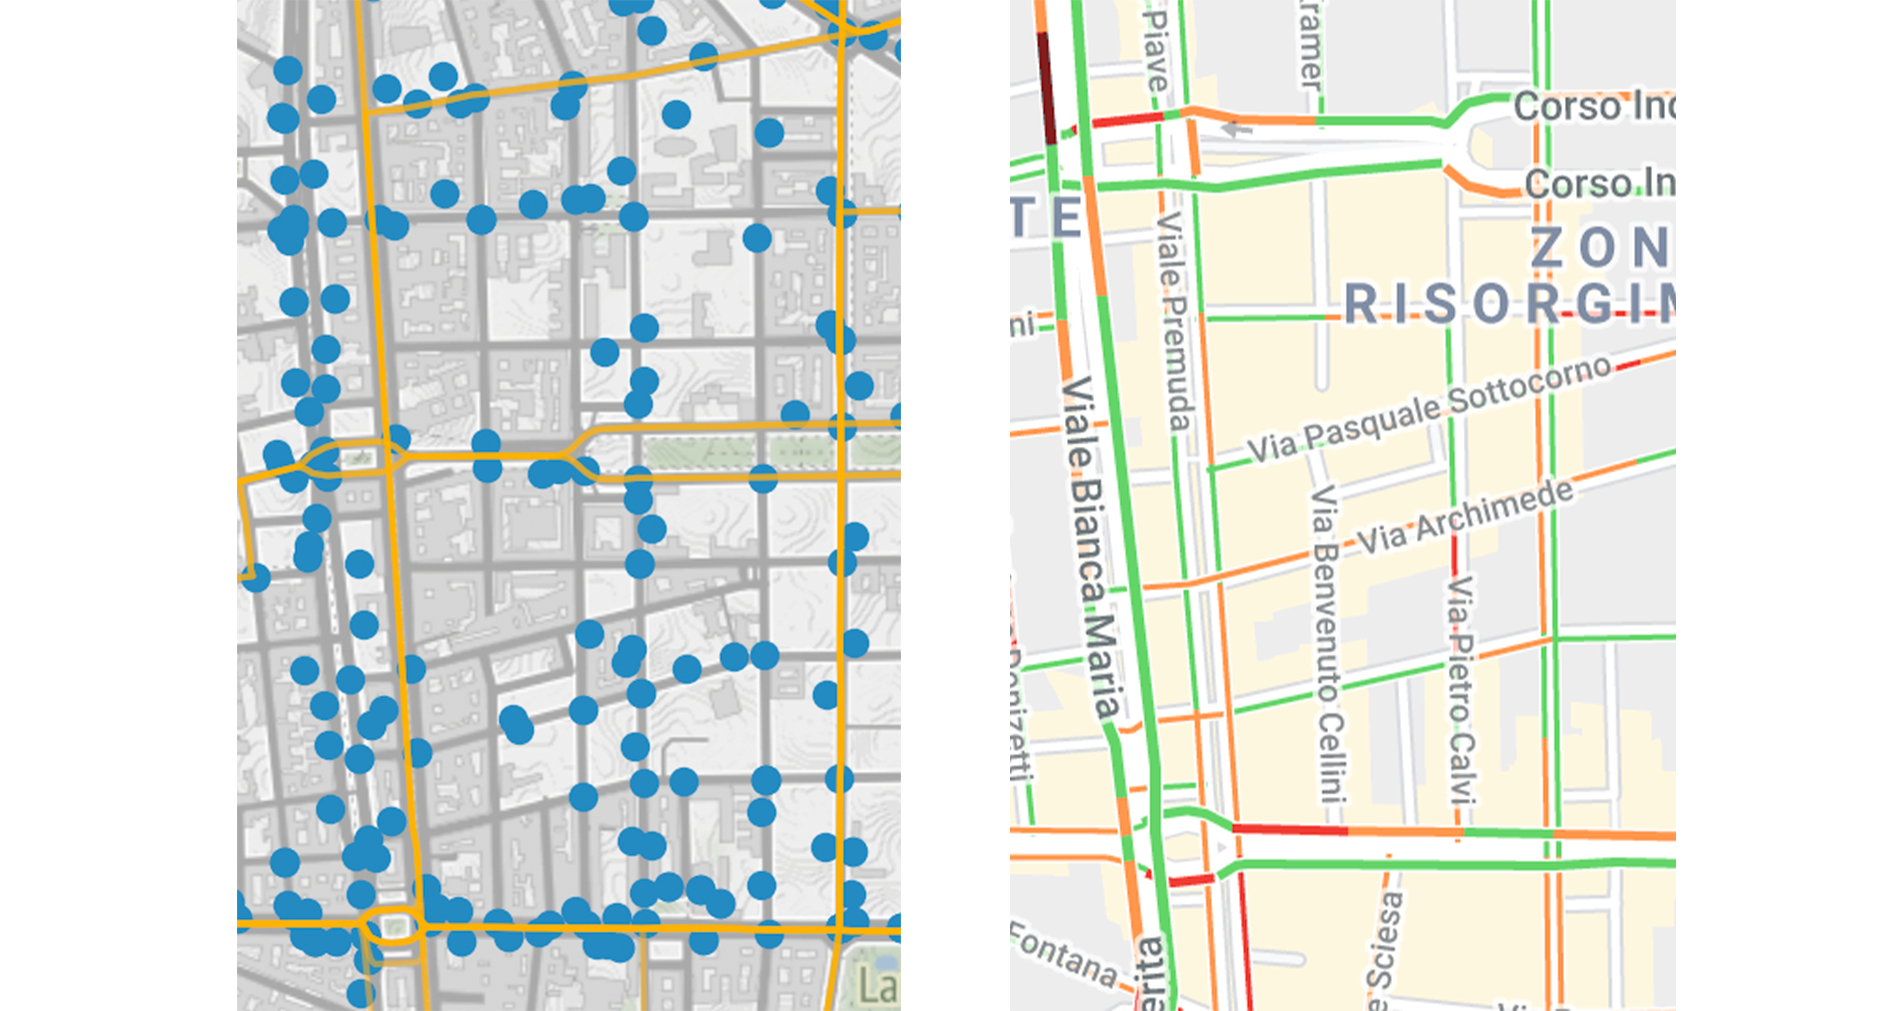
\includegraphics[width=\linewidth]{../src/atm/22_marzo.png}
    \caption{Linee Autobus e Tram a Milano}
    \label{fig:22_marzo}
\end{figure}
%\ref{fig:22_marzo}


%...

%\clearpage
\subsection{Il Pavè influisce sull'incidentalit\'a?}
Spesso le linee di tram coincidono con strade in pavè
%...
Servirebbe una mappa delle strade in pavè a Milano..

\begin{figure}
    \includegraphics[width=\linewidth]{../dataset/pave/Cartina_Milano_Strade_Pavimentazione_Pavé_2.jpg}
    \caption{Cartina con strade in pavè a Milano}
    \label{fig:pave_milano}
\end{figure}

%\ref{fig:pave_milano}

%\clearpage
\section{Incidenti e Piste  Ciclabili}

%\clearpage
\section{Incidenti e Autovelox}

Per sapere se gli autovelox hanno influenza sull'incidentalit\'a, 
bisognerebbe innanzi tutto sapere quando sono stati posizionati i dispositivi, e solo a quel punto, 
avendo dati su incidenti prima e dopo l'installazione, sarebbe possibile trarre conclusioni.

Alcuni dati sull'installazione di autovelox esistono per l'anno 2014, tuttavia i dati 
riguardo agli incidenti sono solo riguardanti l'anno 2016, in quanto Istat non ha rilasciato 
le posizioni degli incidenti in altre annate.

% TODO: devo scrivere come ho ricavato le posizioni degli autovelox installati nel 2014?
% (sono individuati tramite label) 


Gli autovelox installati nel 2014, presenti nel dataset, sono rappresentati nella seguente mappa.
\begin{figure}
    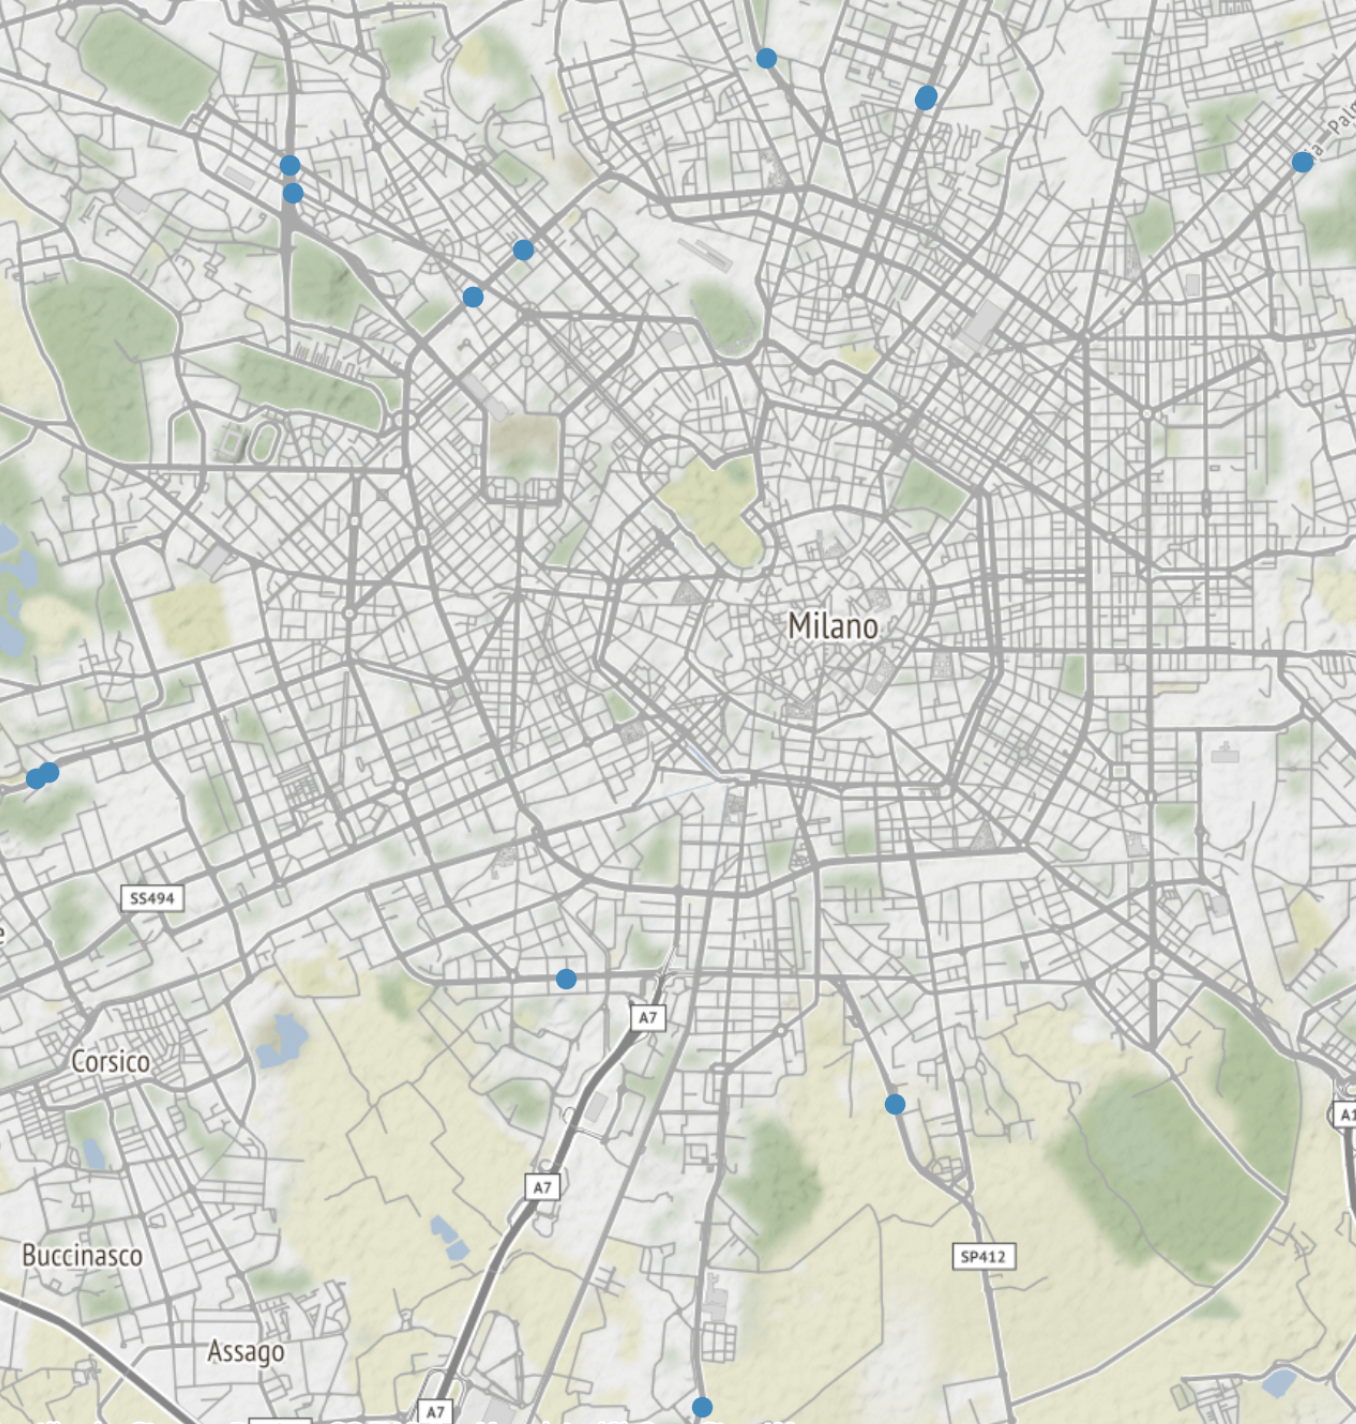
\includegraphics[width=\linewidth]{../src/autovelox/autovelox_2014.png}
    \caption{Autovelox installati nel 2014}
    \label{fig:autovelox_2014}
\end{figure}

%\ref{fig:autovelox_2014}

è comunque possibile sovrapporre i dataset, per vedere se gli autovelox hanno un qualche tipo di 
effetto sugli incidenti.

\begin{figure}
    \includegraphics[width=\linewidth]{../src/autovelox/mappa_3.png}
    \caption{Autovelox e Incidenti a Milano}
    \label{fig:autovelox}
\end{figure}

%\ref{fig:autovelox}

%...


%\clearpage
\section{Incidenti e Meteo}

%%%%%%%%%%%%%%%%%%%%%%%%%%%%%%%%%%%%%%%%%%%%%%%%%%%%%%
%\clearpage
\chapter{Dati su Incidenti}

Per quanto riguarda dati generali su incidenti in Italia, sono disponibili due dataset molto ampi, 
il primo, rilasciato da Istat, contiene dati dal 2010 al 2018 che riguardano campi come data, ora, 
numero di persone a bordo, tipo di incrocio, tipo di veicolo, ecc..
Il secondo è invece messo a disposizione da Automobile Club D'Italia (ACI) che contiene dati simili, 
ma in più mette a disposizione il luogo dell'incidente, come autostrada o strada provinciale.

%\clearpage
\section{Dati Istat su veicoli}

Il dataset Istat contiene molte informazioni riguardanti i conducenti dei veicoli coinvolti 
nell'incidente, oltre al tipo di veicoli.

%\clearpage
\subsection{Come cambia il tipo di veicolo al cambiare del tipo di strada?}

\begin{figure}
    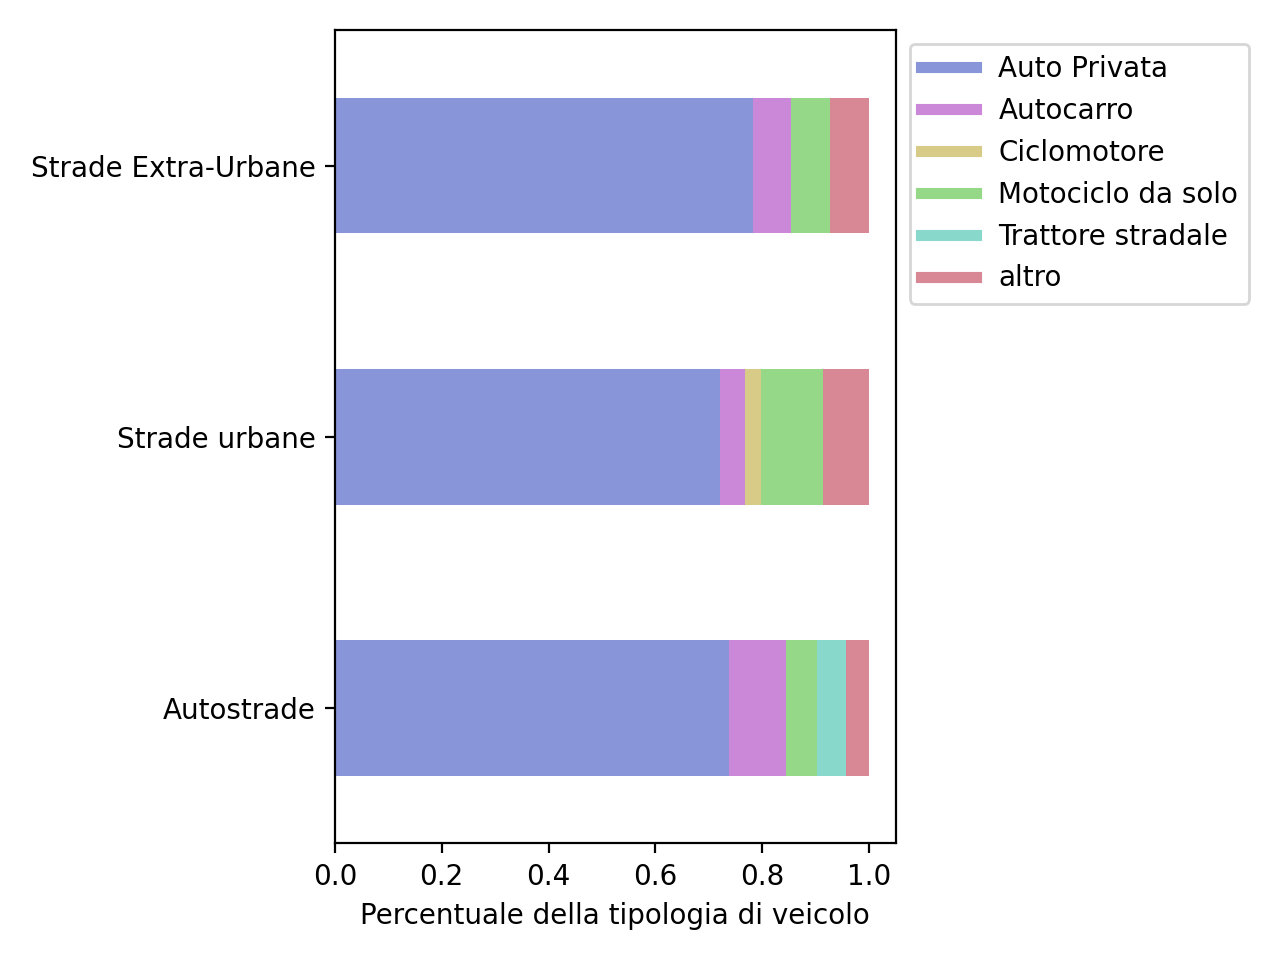
\includegraphics[width=\linewidth]{../src/incidenti/incidenti_senza_coords/tipo_veicoli/differenza_strade.png}
    \caption{Incidenti per tipo di veicolo nel 2010}
    \label{fig:differenza_strade}
\end{figure}

%\ref{fig:differenza_strade}

è possibile notare che, nonostante le auto private siano di gran lunga il tipo di veicolo 
più coinvolto in incidenti, nelle autostrade non sono presenti incidenti con velocipedi, 
anche il numero di incidenti con motocicli è ridotto, mentre cresce molto nelle strade urbane.


%\clearpage
\section{Dati Istat su conducente}

%\clearpage
\subsection{Come cambia il sesso del conducente al cambiare della strada?}

\begin{figure}
    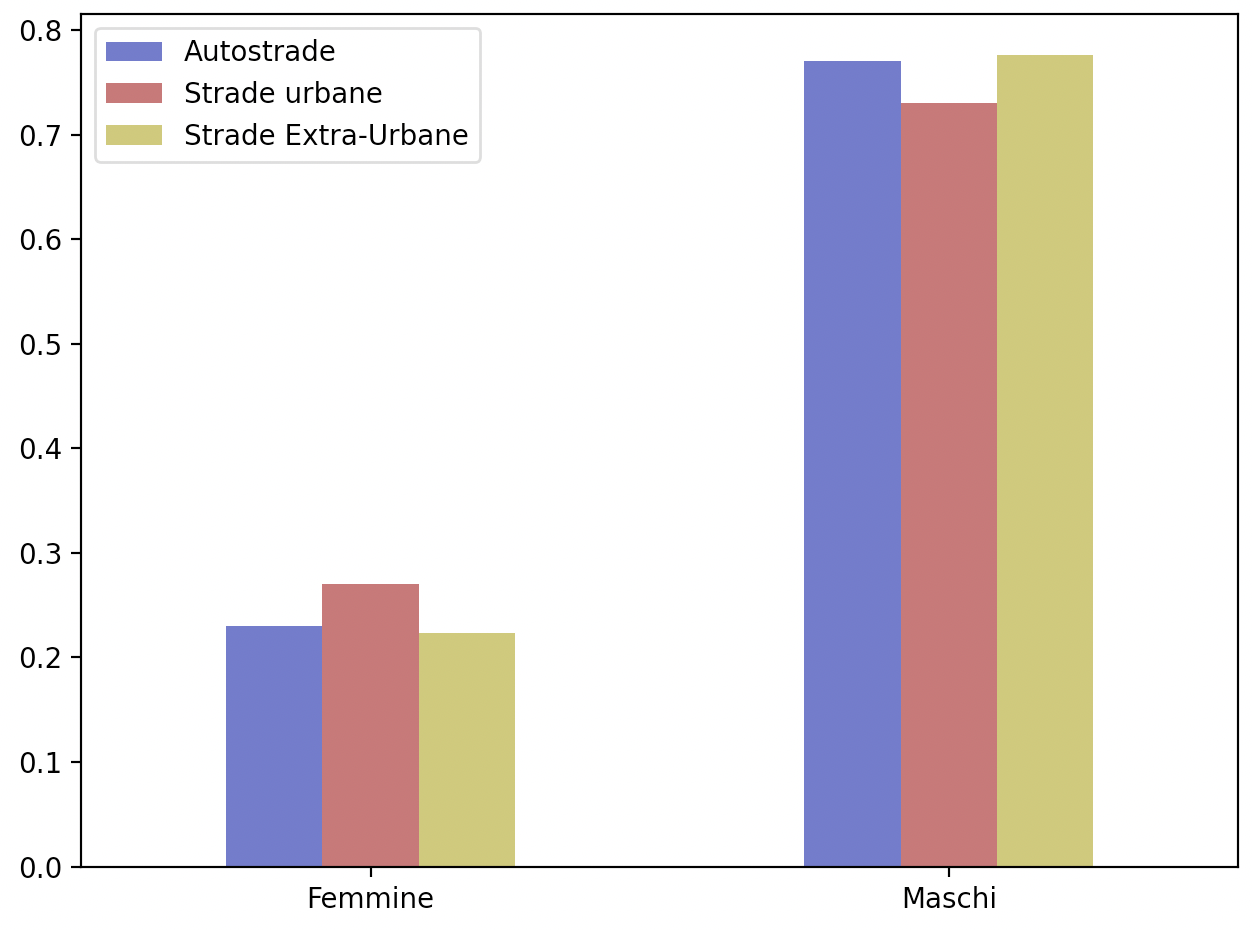
\includegraphics[width=\linewidth]{../src/incidenti/incidenti_senza_coords/tipo_veicoli/uomo-donna.png}
    \caption{Sesso del conducente per tipo di veicolo nel 2010}
    \label{fig:differenza_uomo_donna}
\end{figure}

%\ref{fig:differenza_uomo_donna}

Il numero di incidenti per genere è tende ad essere 75\% circa uomini e 25\% donne.
Nelle strade  urbane, la percentuale di incidenti con conducente donna aumenta leggermente nel 2010, 
questo vale per tutti gli anni?

%TODO: stima della percentuale di conducenti maschi/femmine


%\clearpage
\subsection{Come cambia l'et\'a del conducente al cambiare della strada?}

\begin{figure}
    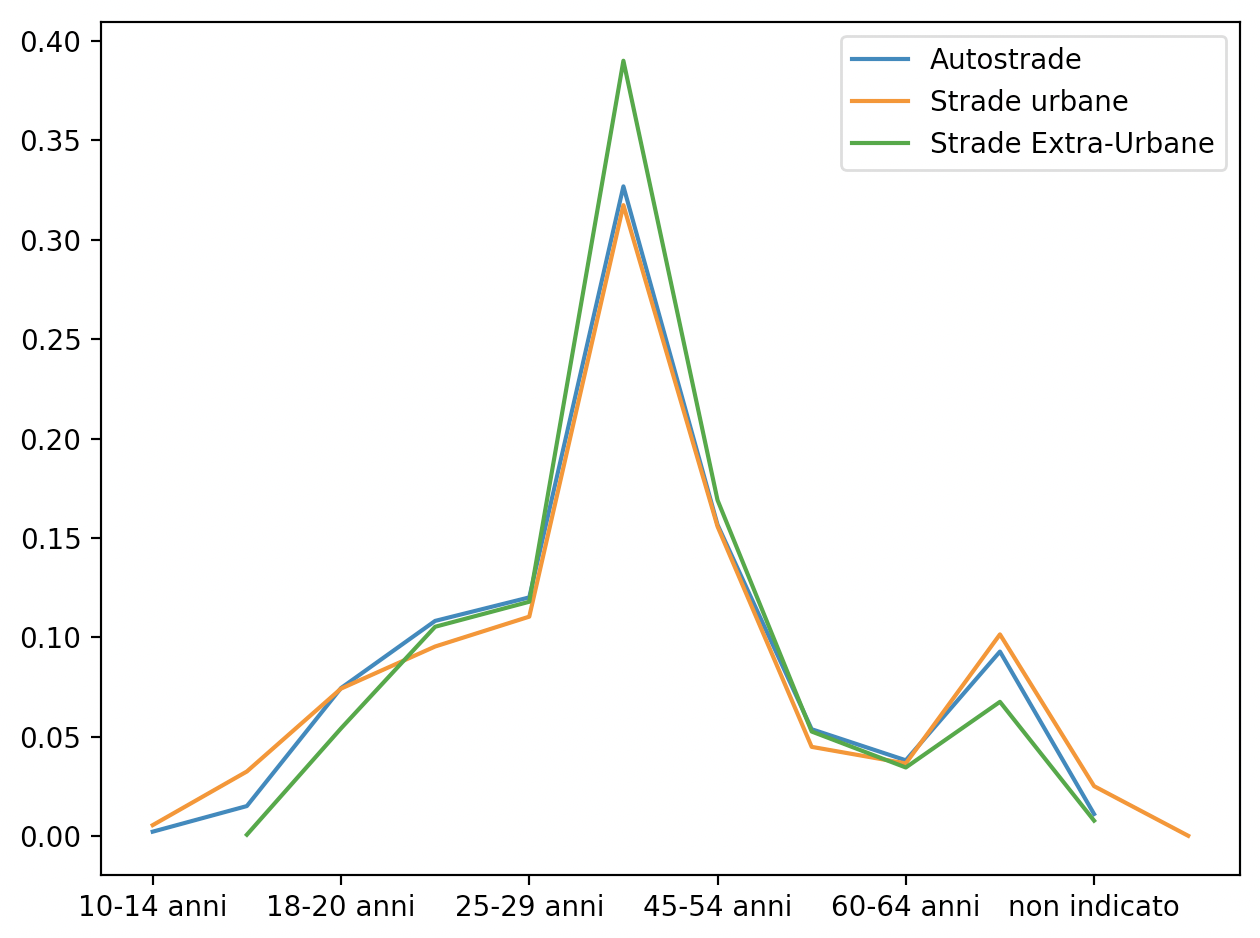
\includegraphics[width=\linewidth]{../src/incidenti/incidenti_senza_coords/tipo_veicoli/differenza_eta.png}
    \caption{Fascia di et\'a del conducente per tipo di veicolo nel 2010}
    \label{fig:differenza_eta}
\end{figure}



Risultati non troppo interessanti\dots

%...

%\clearpage
\subsection{Il numero di passeggeri influisce sull'incidentalit\'a?}

\begin{figure}
    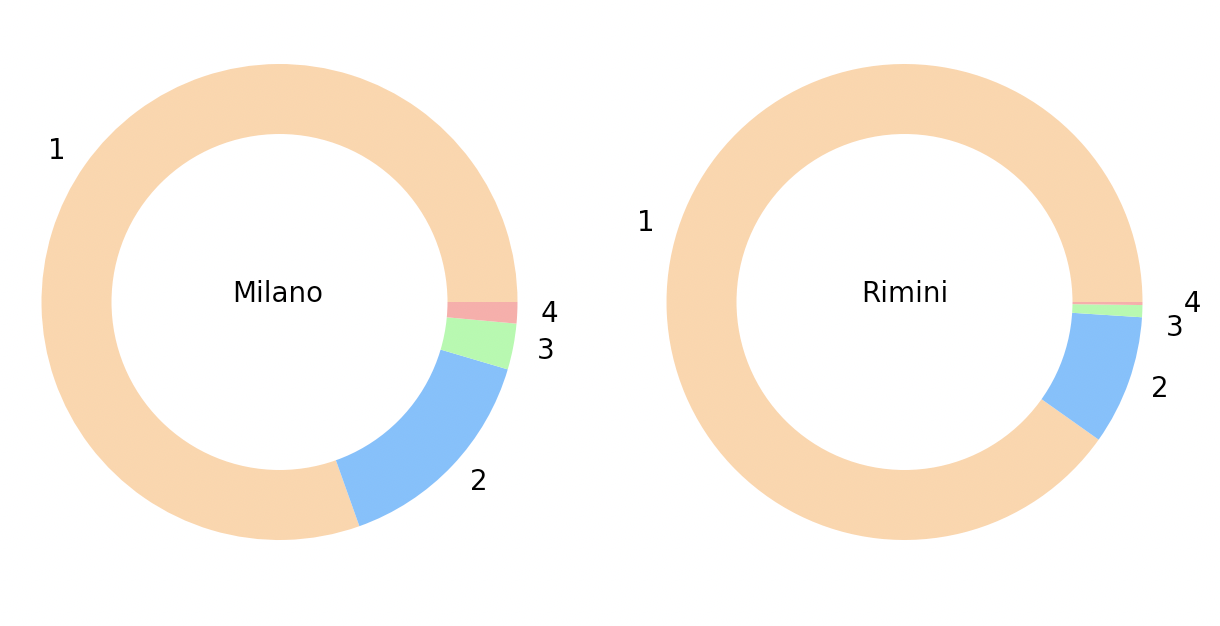
\includegraphics[width=\linewidth]{../src/incidenti/incidenti_senza_coords/tipo_veicoli/passeggeri.png}
    \caption{Numero di passeggeri in incidenti per Milano e Rimini}
    \label{fig:passeggeri_milano_rimini}
\end{figure}

La maggior parte degli incidenti sembra avvenire quando in macchina è presente solo il conducente.
Si sono prese in considerazione le provincie di Milano e Rimini, per controllare se la localit\'a 
marittima influisse sul numero di incidenti, ma sembra che quest'ultima abbia una percentuale 
ancora più alta di incidenti in cui è presente solo il conducente, rispetto a Milano.

%\clearpage
\subsection{Il conducente se da solo si distrae con il telefono cellulare?}

Per quanto non siano disponibili dati su questo ambito, si potrebbe confrontare gli anni tra 2010 e 2013, 
in cui l'uso del cellulare in macchina ancora non era frequente, rispetto agli anni più recenti.

%...


%\clearpage
\section{Dati Istat su orari e mesi}

%\clearpage
\subsection{Quanto influiscono le ore di punta sull'incidentalit\'a?}

Per prima cosa, con un semplice conto degli incidenti durante il weekend 
e confrontandolo con il numero di quelli avvenuti durante la 
settimana lavorativa, si osserva che nel weekend avvengon più incidenti 
durante la sera e la notte, mentre durante la settimana in giornata.

\begin{figure}
    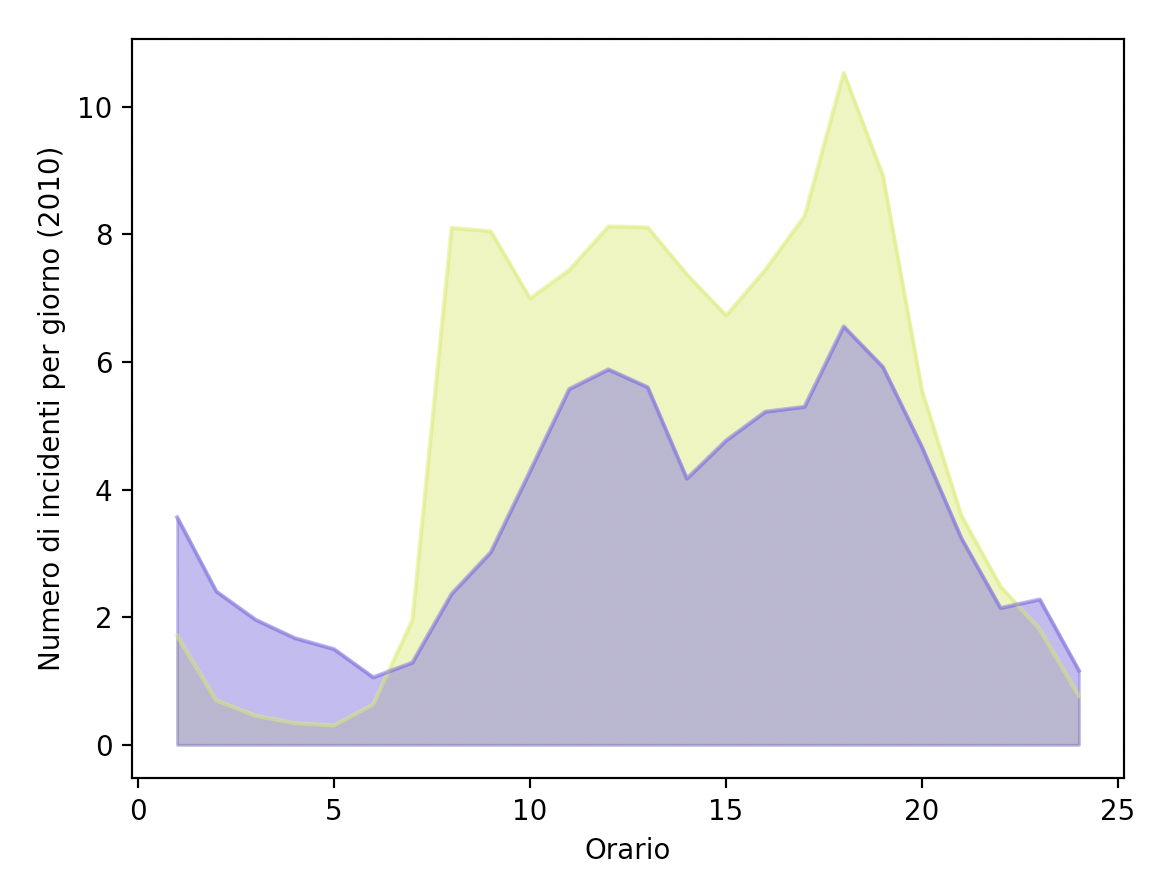
\includegraphics[width=\linewidth]{../src/incidenti/incidenti_senza_coords/ore_punta/week_weekend.png}
    \caption{Incidenti per ora}
    \label{fig:week_weekend}
\end{figure}

Per quanto riguarda gli orari di punta, 
sono state prese in considerazione due fasce orarie, la prima, 
mattutina dalle 7:00 alle 10:00, e la seconda pomeridiana, 
dalle 17:00 alle 19:00

% Tolti perchè ripetevano dati già visti
%\begin{figure}
%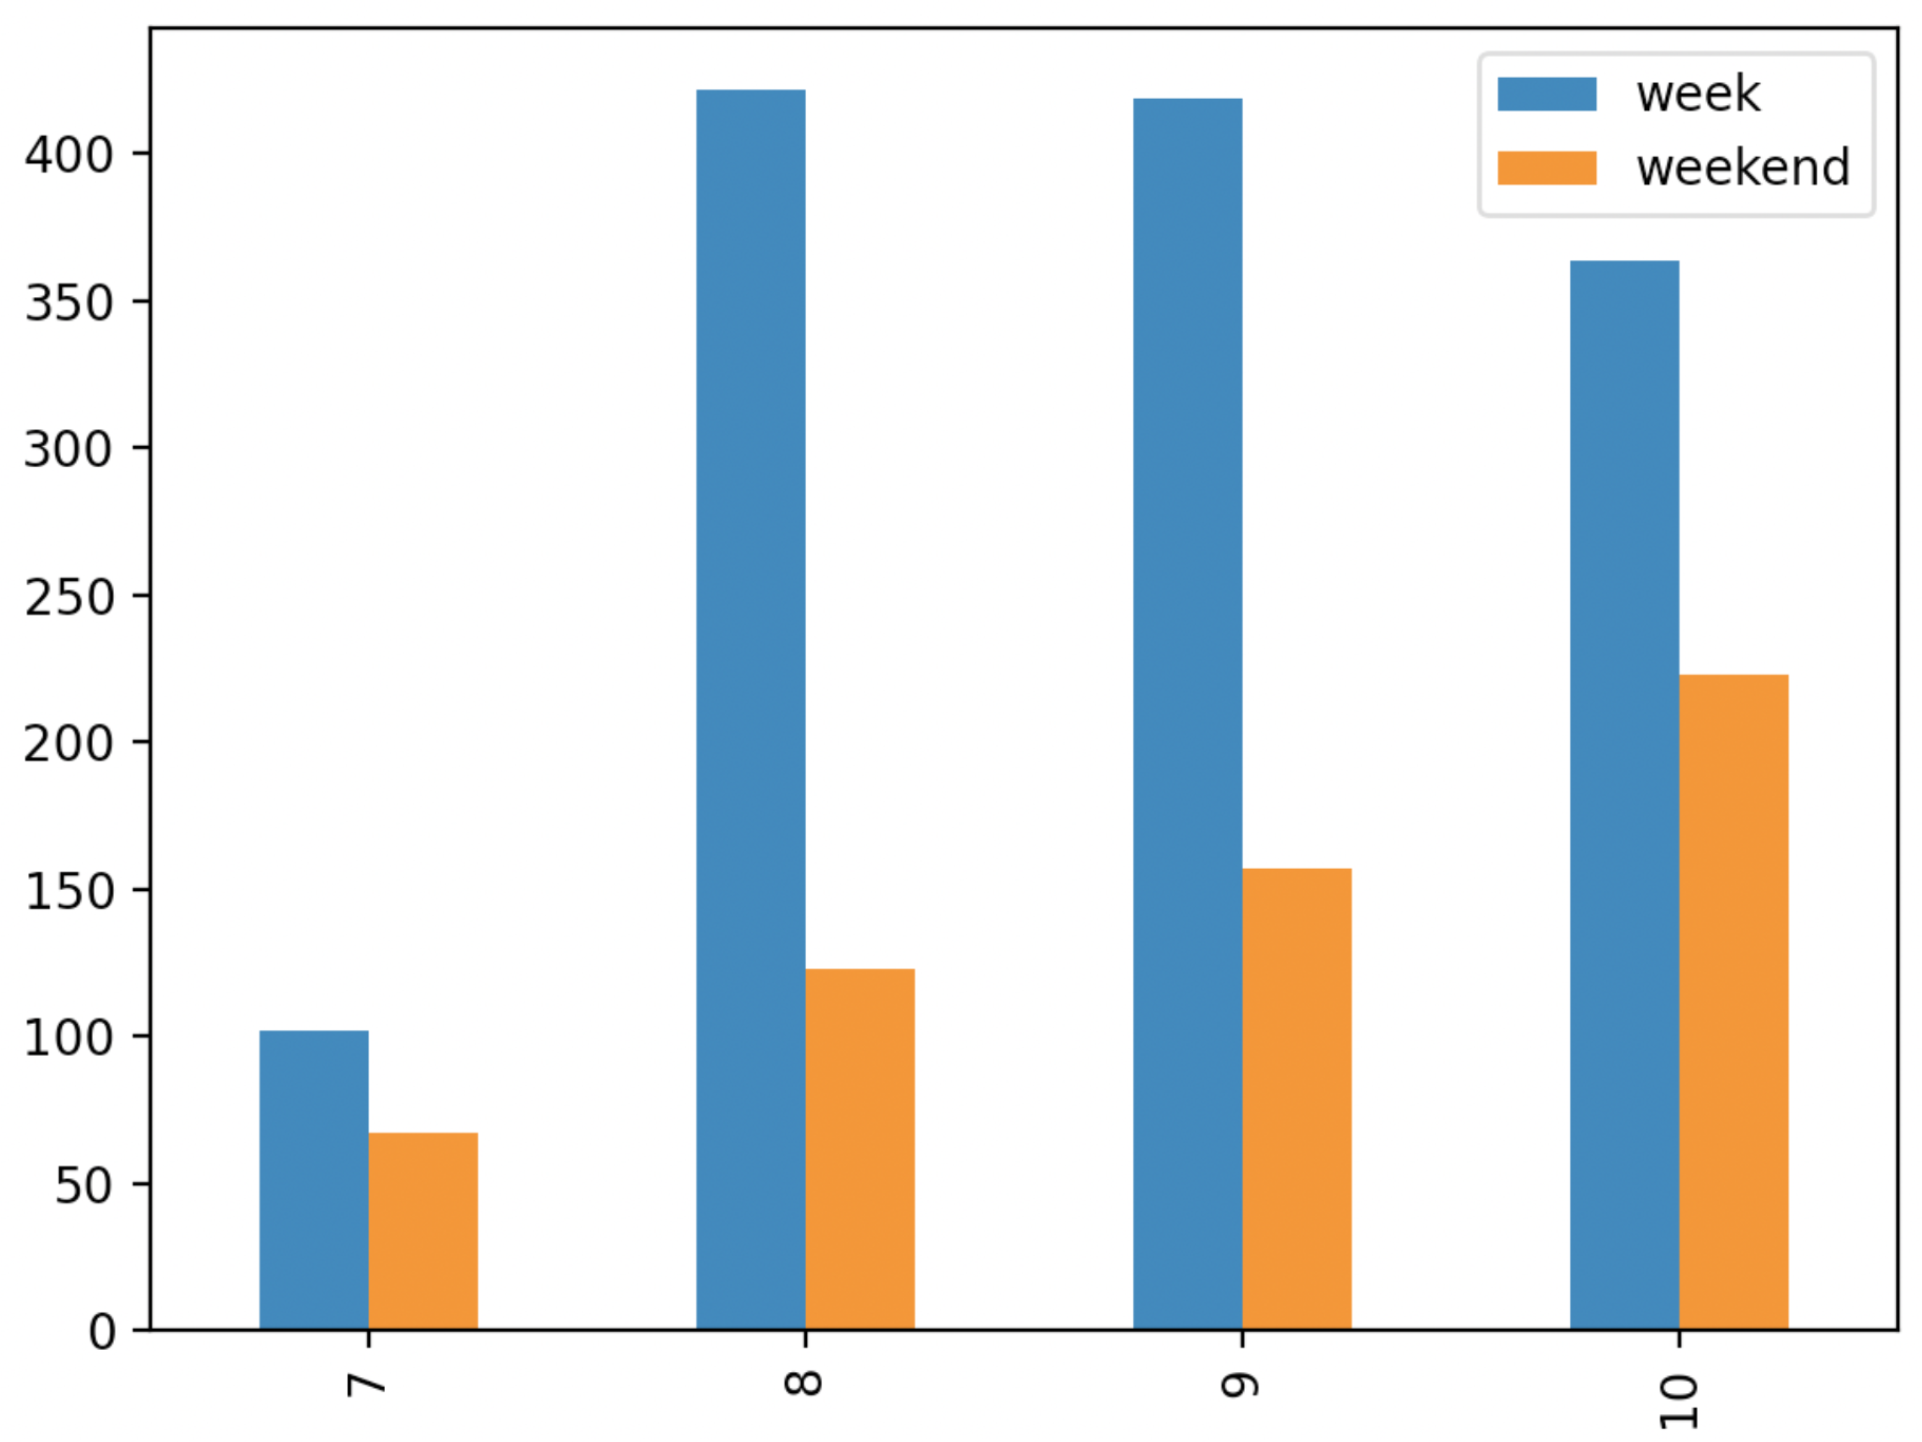
\includegraphics[width=\linewidth]{../src/incidenti/incidenti_senza_coords/ore_punta/ore_punta_mattina.png}
%\caption{Ore di punta Mattutine}
%\label{fig:punta_mattina}
%\end{figure}
%
%\begin{figure}
%    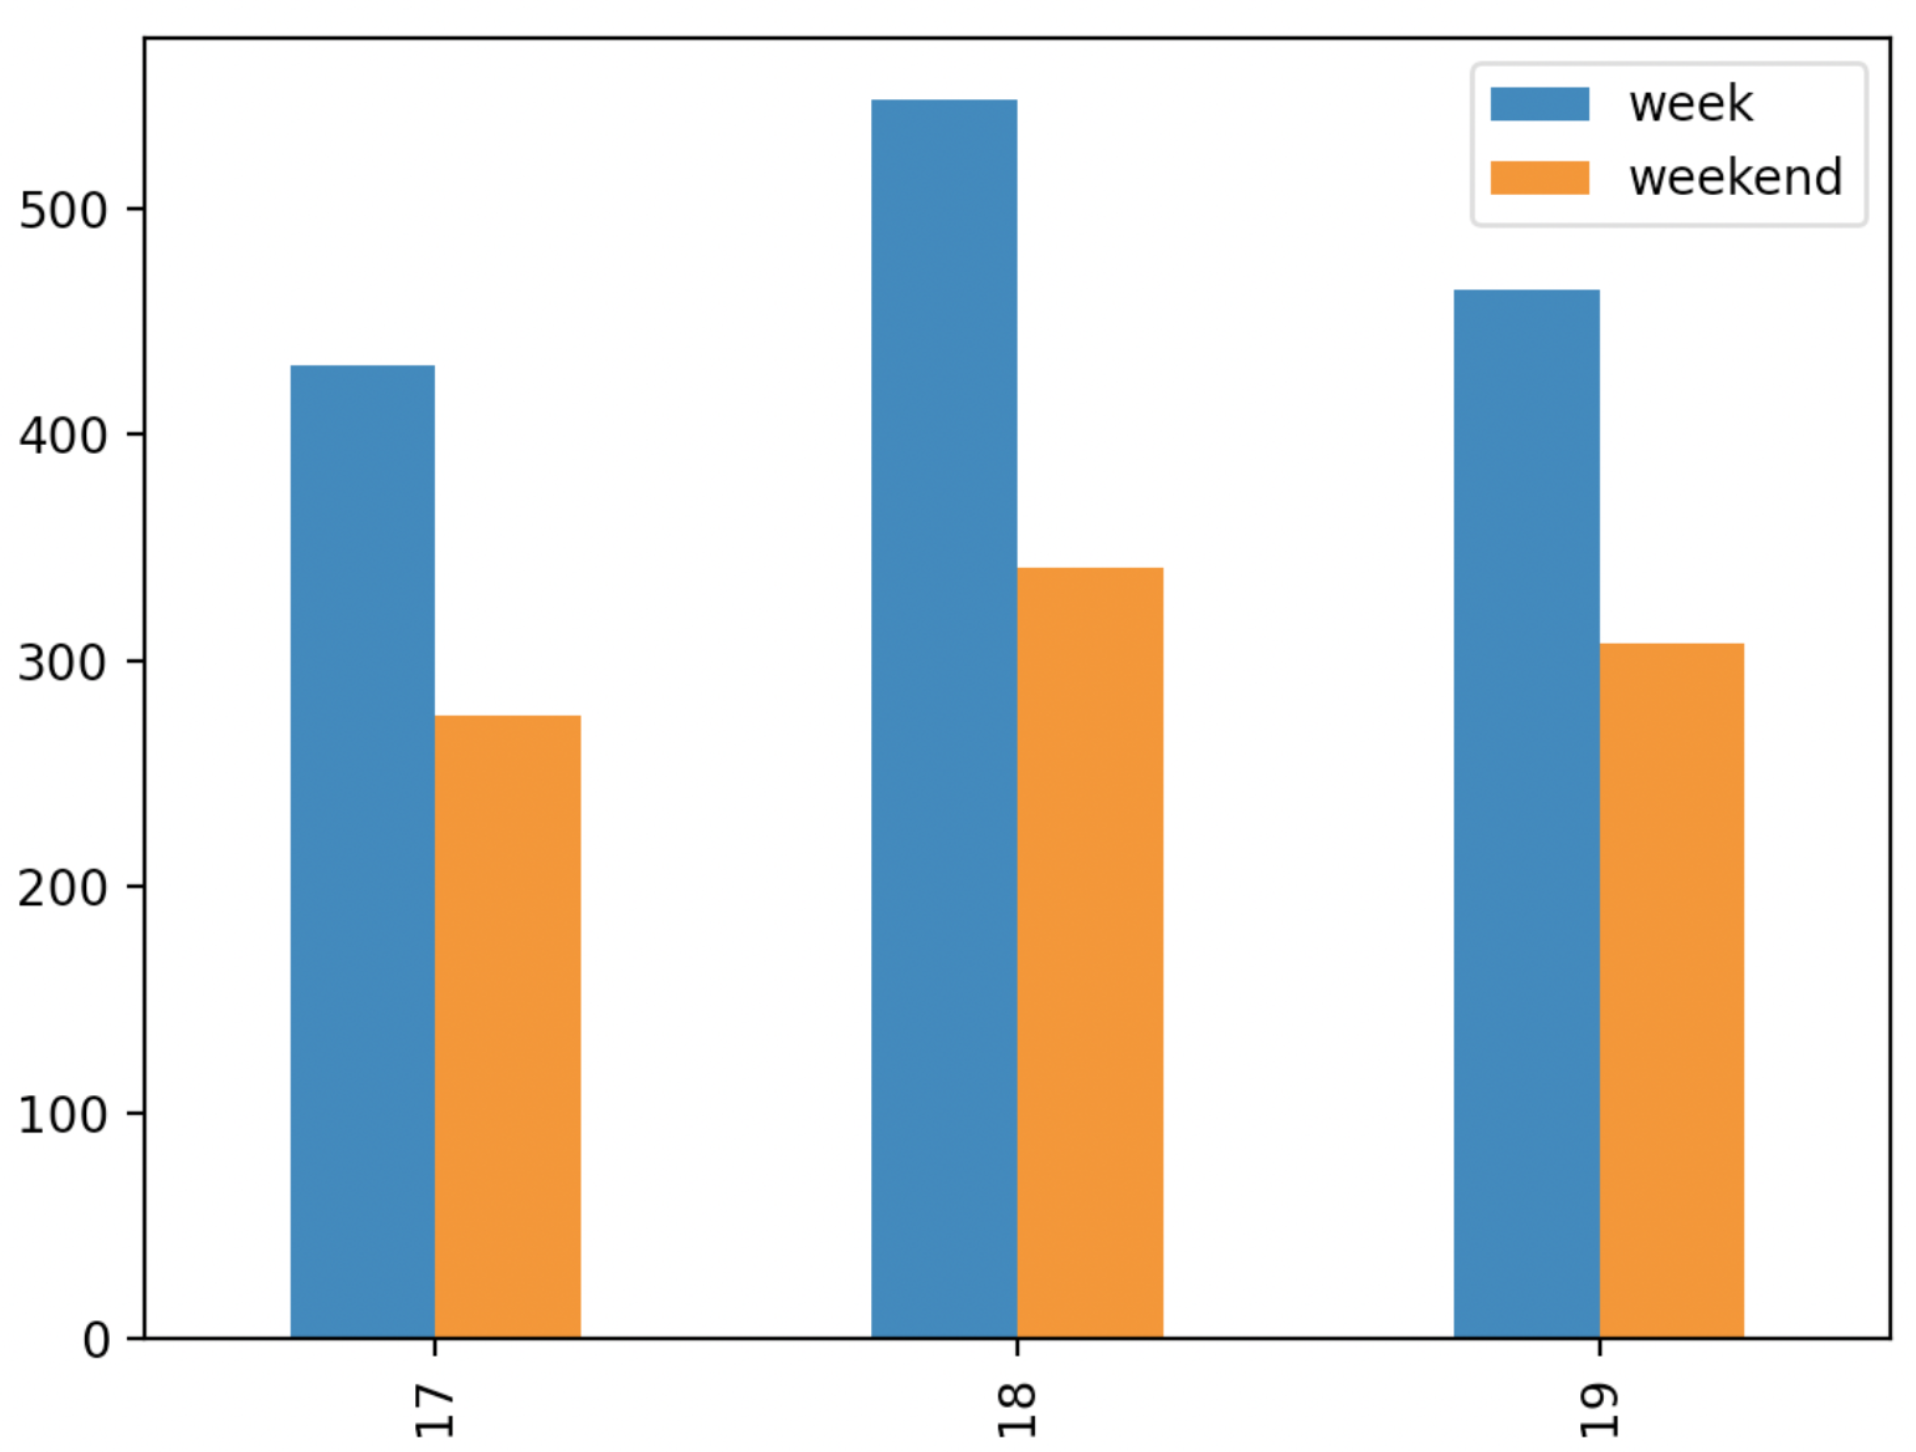
\includegraphics[width=\linewidth]{../src/incidenti/incidenti_senza_coords/ore_punta/ore_punta_sera.png}
%    \caption{Ore di punta serali}
%    \label{fig:punta_sera}
%\end{figure}


Va sottolineato che i grafi indicano gli incidenti normalizzati per numero di 
giorni, 
quindi gli incidenti totali della settimana sono divisi per cinque giorni, 
mentre quelli del weekend per due.
Si pu\'o osservare che nella fascia oraria delle 18:00, 
avvengono molti più sinistri, mentre nella fascia mattutina, 
il numero non sembra variare molto dalla media di incidenti durante il giorno.

%\clearpage
\subsection{è possibile accentuare le ore di punta mattutine?}

Se si selezionano solo gli incidenti nella provincia di Milano, è possibile individuare 
il secondo picco di incidenti, quello durante le ore di punta mattutine

\begin{figure}
    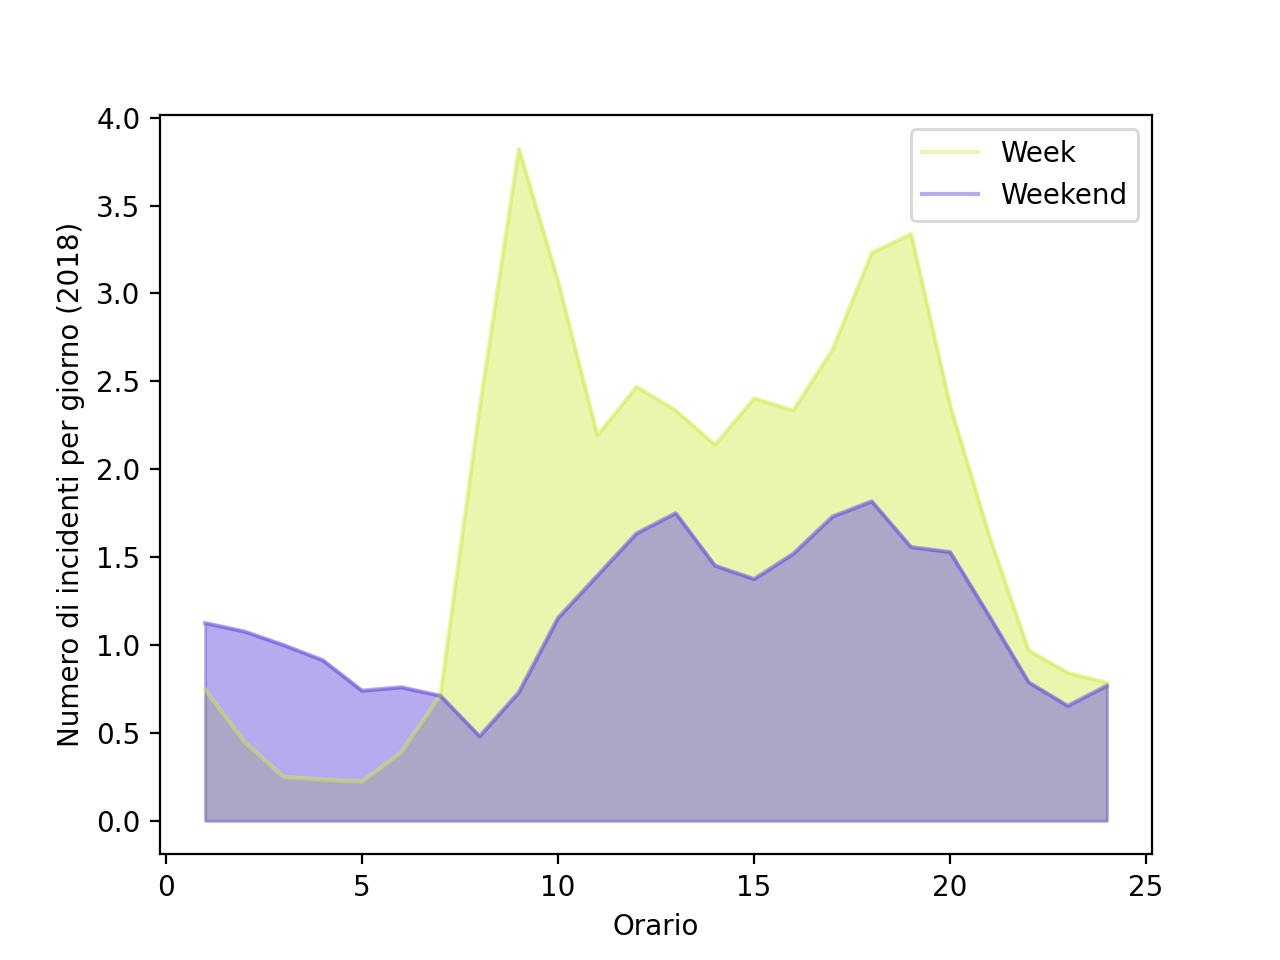
\includegraphics[width=\linewidth]{../src/incidenti/incidenti_senza_coords/ore_punta/week_weekend_milano.png}
    \caption{Incidenti per ora a Milano}
    \label{fig:week_weekend_milano}
\end{figure}

%...

%\clearpage
\subsection{Si ha la stessa tendenza di notte?}

\todo{reference a immagine fig:week\_weekend}
Come individuato dal primo grafo in \textit{week\_weekend}, durante le 
ore notturne si ha la tendenza opposta.

\begin{figure}
    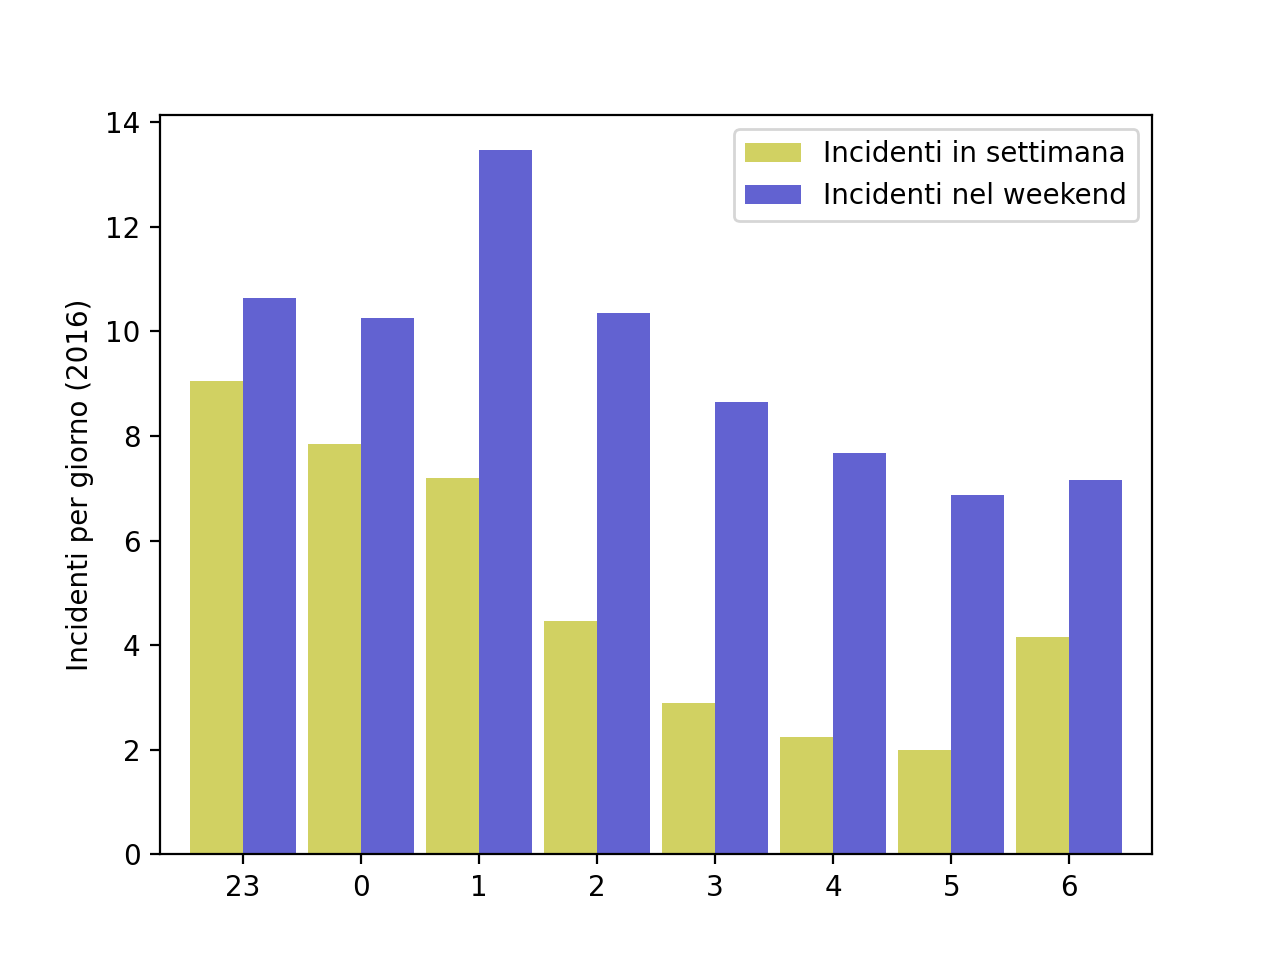
\includegraphics[width=\linewidth]{../src/incidenti/incidenti_senza_coords/ore_punta/ore_notte.png}
    \caption{Incidenti durante ore serali o notturne}
    \label{fig:ore_notte}
\end{figure}

%...

%\clearpage
\subsection{Quanto influiscono le vacanze estive sull'incidentalit\'a?}

\begin{figure}
    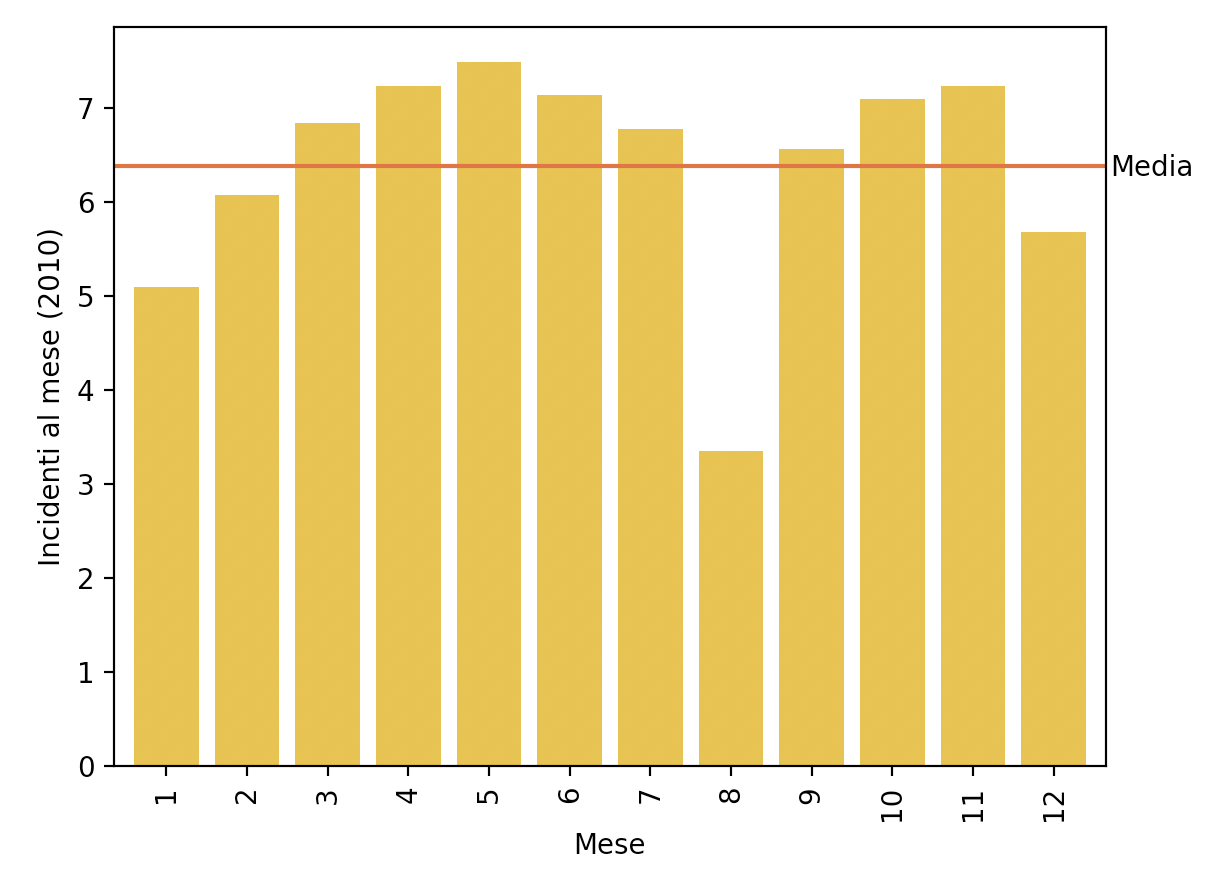
\includegraphics[width=\linewidth]{../src/incidenti/incidenti_senza_coords/mese_incidenti/milano_mese.png}
    \caption{Incidenti per mese in Milano}
    \label{fig:milano_mese}
\end{figure}

Si nota un chiaro calo di incidenti nel mese di Agosto in provincia di Milano.
\'E possibile controllare il decremento del numero di incidenti, anche per gli altri anni, 
in cui sono disponibili dati.

\begin{center}
    \def\arraystretch{1.5}%  
    \begin{tabular}{ |c|c| } 
    \hline
    Anno & Incremento in Agosto \\ 
    \hline
    2010 & -47.4\%  \\ 
    2011 & -35.14\% \\
    2012 & -45.46\% \\
    2013 & -41.37 \% \\
    \hline
    \end{tabular}
\end{center}

Per quanto riguarda gli anni successivi, il dataset non dispone più di un campo che indichi il mese 
dell'incidente, ma è disponibile soltanto il trimestre.

\todo{Aggiungo tabella per trimestre?}

Per quanto possano esserci molti fattori che contribuiscono a questa tendenza, 
quello che influisce di più devono essere le partenze per le vacanze.

%\clearpage
\subsection{è possibile individuare la tendenza inversa in localit\'a  di mare?}

\begin{figure}
    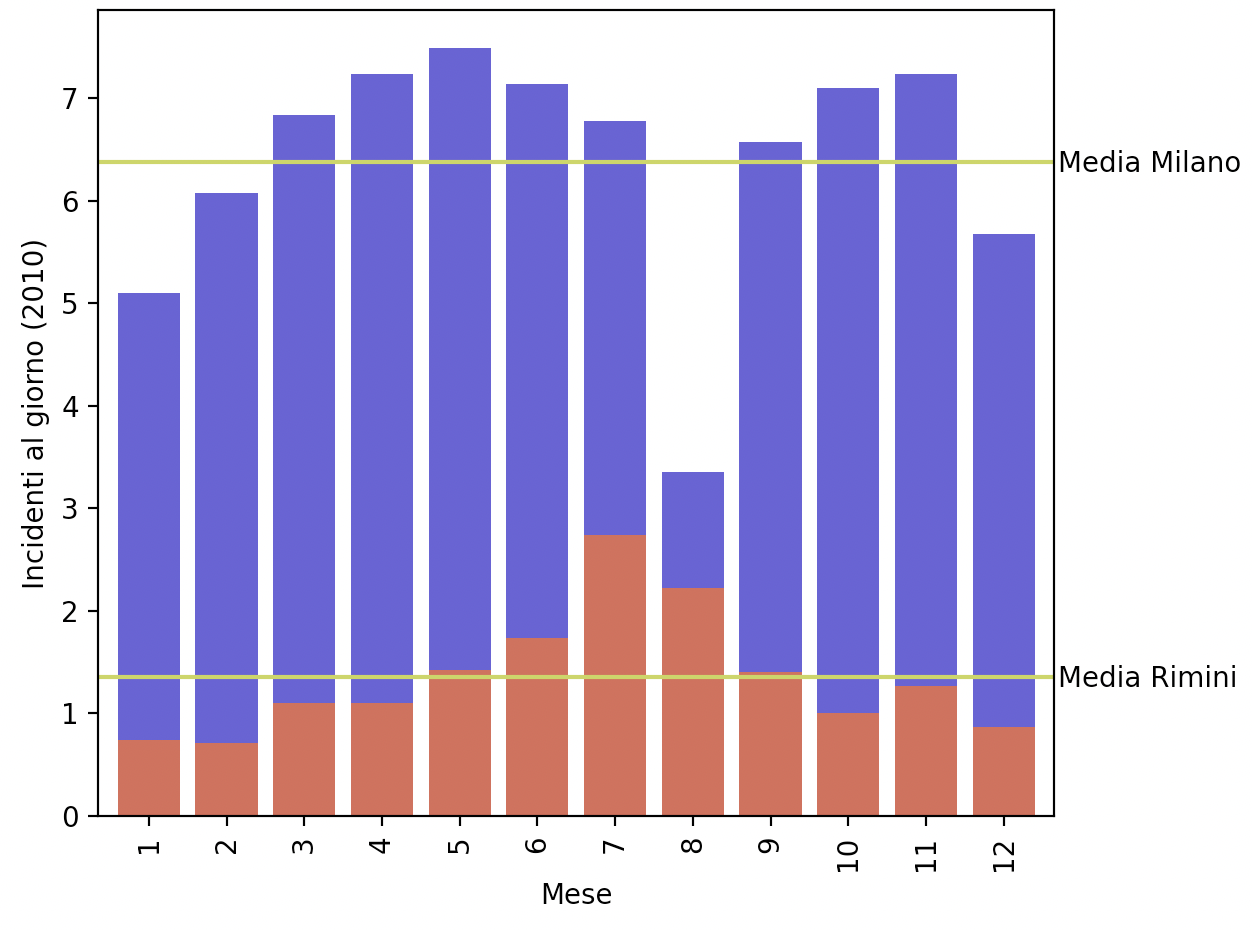
\includegraphics[width=\linewidth]{../src/incidenti/incidenti_senza_coords/mese_incidenti/milano_rimini.png}
    \caption{Incidenti per mese in Milano e Rimini}
    \label{fig:milano_rimini}
\end{figure}

L'unica localit\'a in cui si è riscontrata la tendenza inversa è in provincia 
di Rimini.

\begin{center}
    \def\arraystretch{1.5}%  
    \begin{tabular}{ |c|c|c| } 
    \hline
    Anno & Agosto & Luglio \\ 
    \hline
    2010 & 63.75\% & 101.72\% \\ 
    2011 & 60.49\% & 54.6 \%  \\
    2012 & 45.93\% & 75.97\%  \\
    2013 & 51.82\% & 116.37\% \\
    \hline
    \end{tabular}
\end{center}

Tuttavia, osservando il grafo equivalente della Valle d'Aosta, è possibile notare 
un notevole incremento di incidenti sia in Gennaio che in Agosto, possibili 
conseguenze, rispettivamente, dell'inizio della stagione sciistica ed estiva.

\begin{figure}
    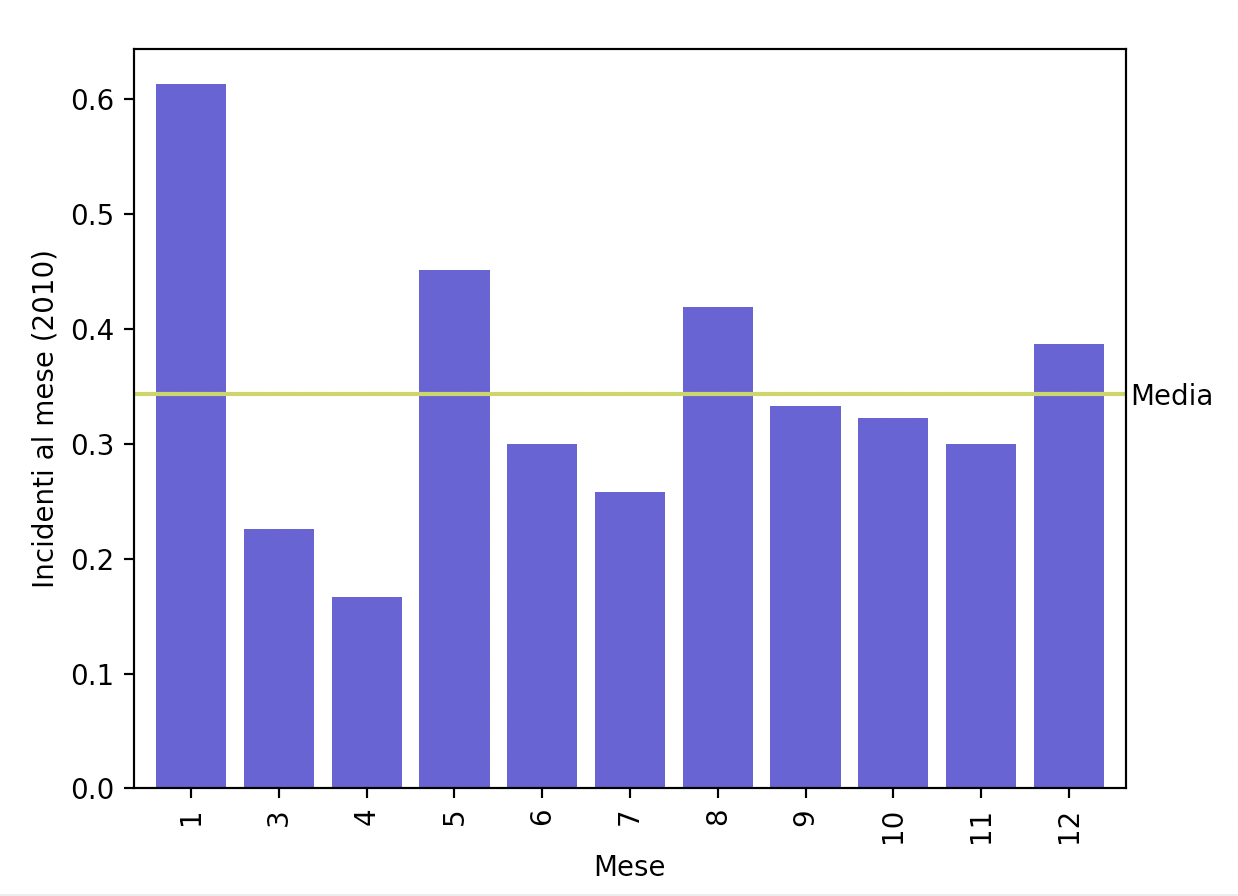
\includegraphics[width=\linewidth]{../src/incidenti/incidenti_senza_coords/mese_incidenti/aosta_mese.png}
    \caption{Incidenti per mese Valle d'Aosta}
    \label{fig:aosta}
\end{figure}

Questa tendenza avviene ogni anno?

\begin{center}
    \def\arraystretch{1.5}%  
    \begin{tabular}{ |c|c|c| } 
    \hline
    Anno & Agosto & Gennaio \\ 
    \hline
    2010 & -2.93 \% & 78.48\%  \\ 
    2011 & 124.0 \% & -32.12\% \\
    2012 & 52.25 \% & -41.44\% \\
    2013 & -15.21\% & -24.63\% \\
    \hline
    \end{tabular}
\end{center}

Il comportamento degli incidenti in Valle d'Aosta è molto inconsistente, soprattutto in Agosto.
Va specificato che la taglia del campione con cui si sta lavorando, per questa provincia, 
è molto piccolo, e sicuramente influisce sulle percentuali di incremento e decremento 
degli incidenti.\\
Nonostane ciò, se si assume che Gennaio 2010 sia un outlier, il numero di incidenti in 
questo mese è sempre in decremento, in modo molto consistente, rispetto alla media.

\todo{Affianco i tre grafi dei trimestri?}
\begin{figure}
    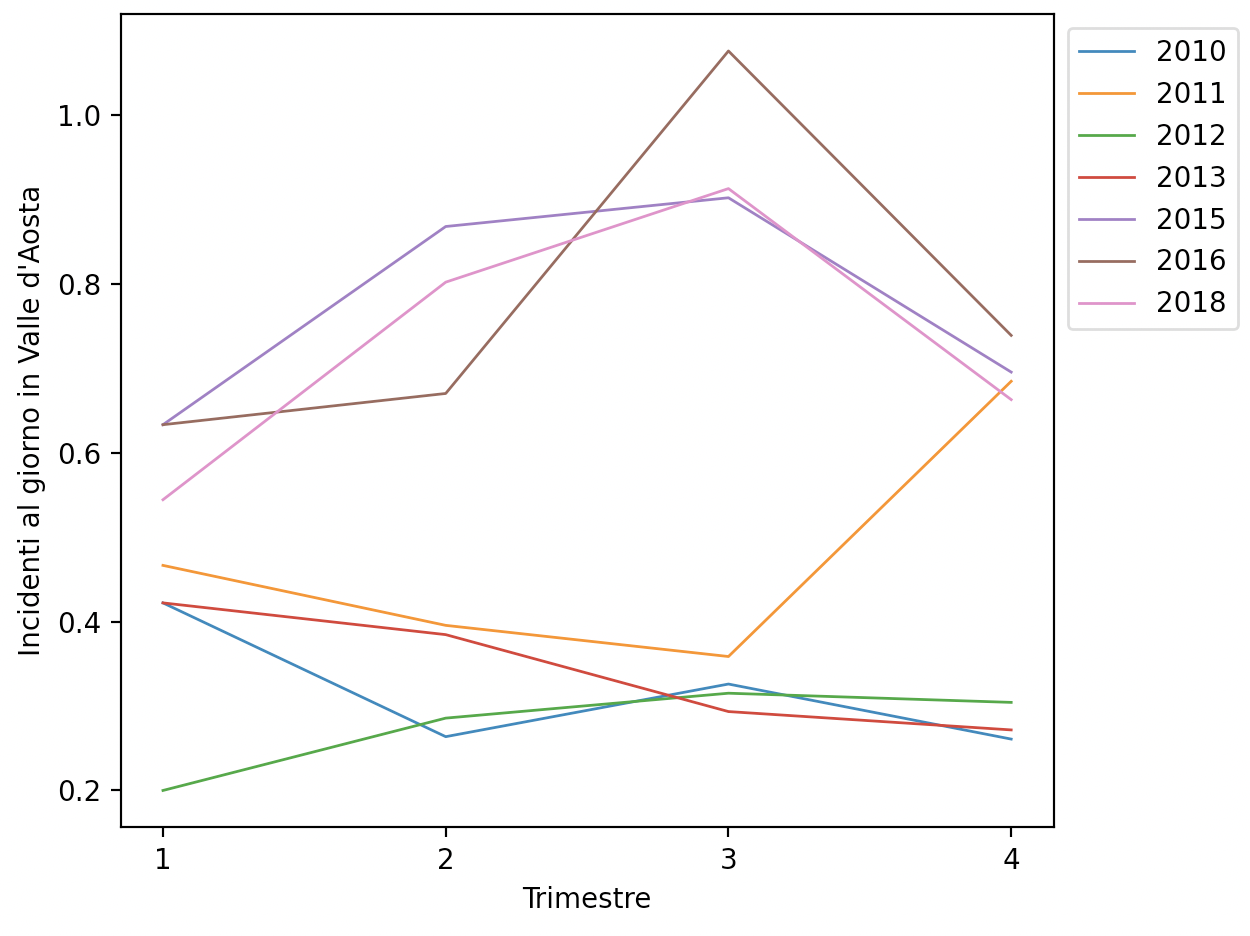
\includegraphics[width=\linewidth]{../src/incidenti/incidenti_senza_coords/mese_incidenti/aosta_timestre.png}
    \caption{Incidenti per trimestre in Valle d'Aosta}
    \label{fig:aosta_trimestre}
\end{figure}

La prima cosa che è possibile notare, è che il picco di Gennaio del 2010 è 
in linea con la tendenza del trimestre invernale. 
Tuttavia, si osserva anche che dall'anno 2015 c'è un ampio gap nel numero di 
incidenti. 
è un cambio di metro di misurazione? 

\begin{figure}
    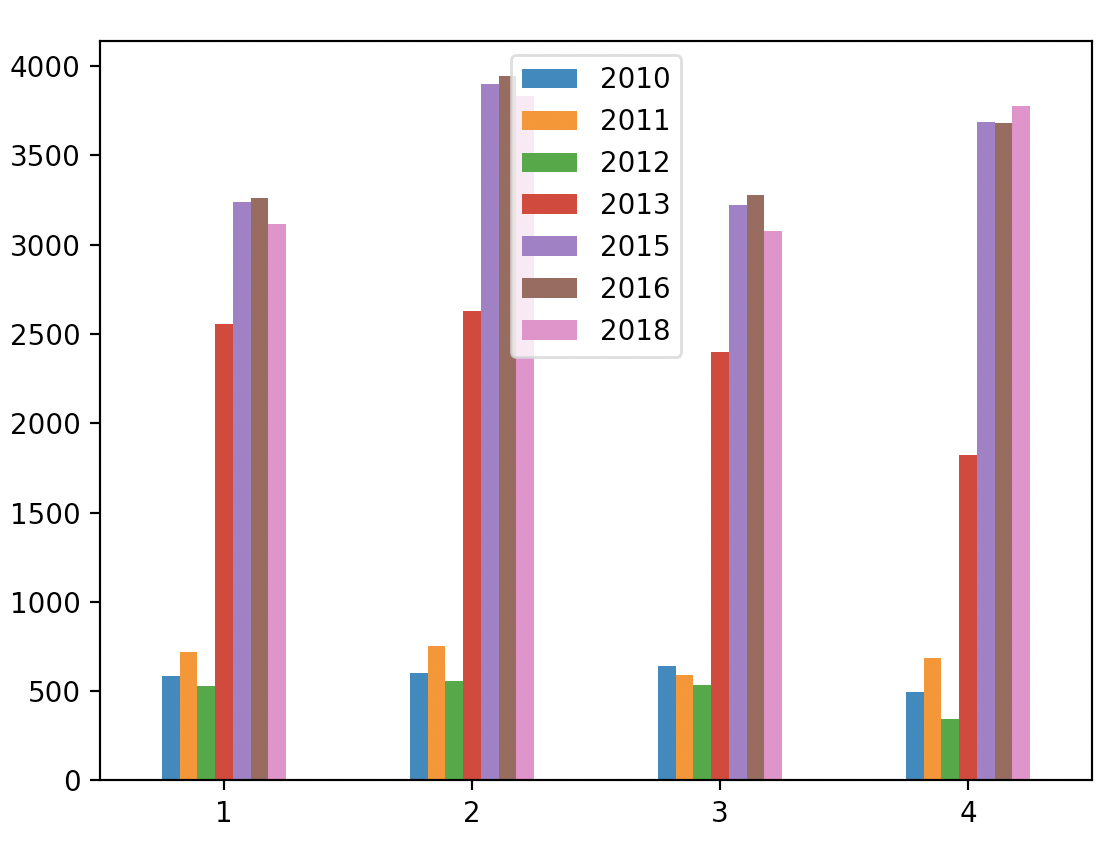
\includegraphics[width=\linewidth]{../src/incidenti/incidenti_senza_coords/mese_incidenti/milano_trimestre.png}
    \caption{Incidenti per trimestre a Milano}
    \label{fig:milano_trimestre}
\end{figure}

\begin{figure}
    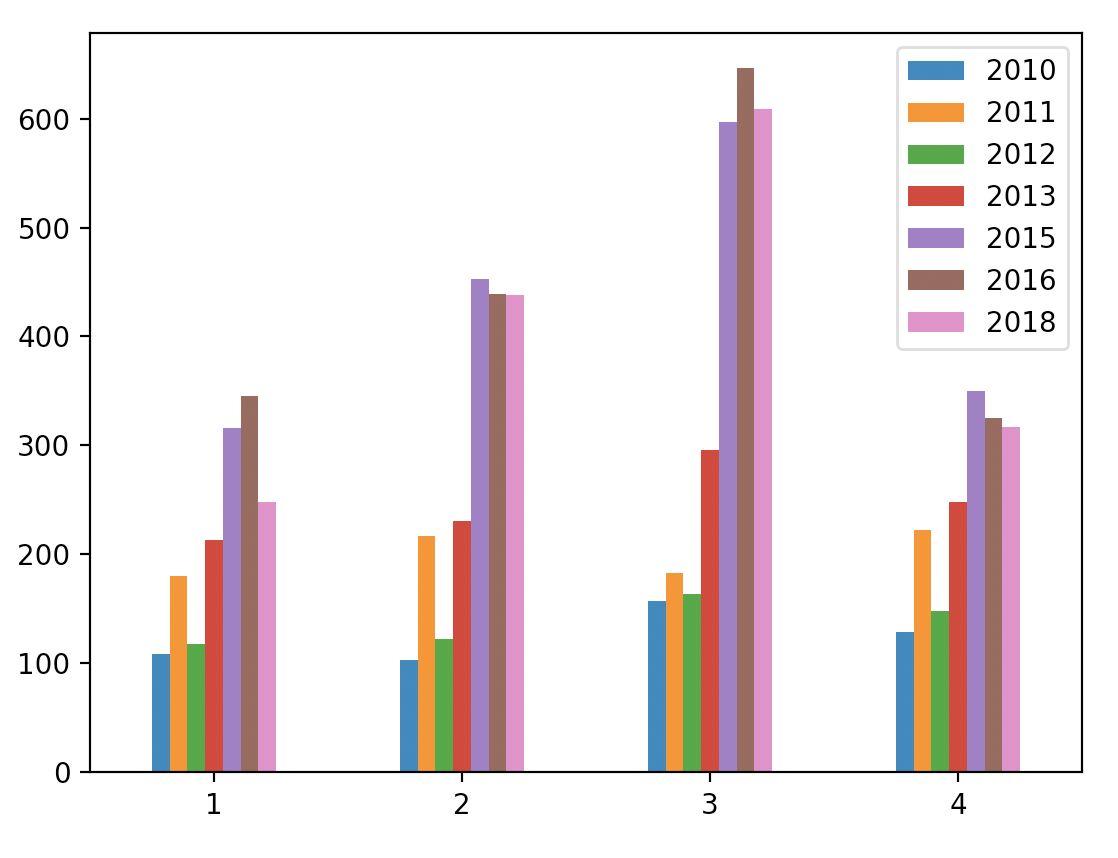
\includegraphics[width=\linewidth]{../src/incidenti/incidenti_senza_coords/mese_incidenti/rimini_trimestre.png}
    \caption{Incidenti per trimestre a Rimini}
    \label{fig:rimini_trimestre}
\end{figure}

I grafi equivalenti di Milano e Rimini mostrano la stessa tendenza di incremento del numero 
di incidenti, ma a Milano, in particolare, il gap sembra essersi 'creato' nel 2013.

%...

%\clearpage
\section{Dati Istat su tipi di incidenti e incroci}

%\clearpage
\subsection{Quali incidenti avvengono con più frequenza?}

\begin{figure}
    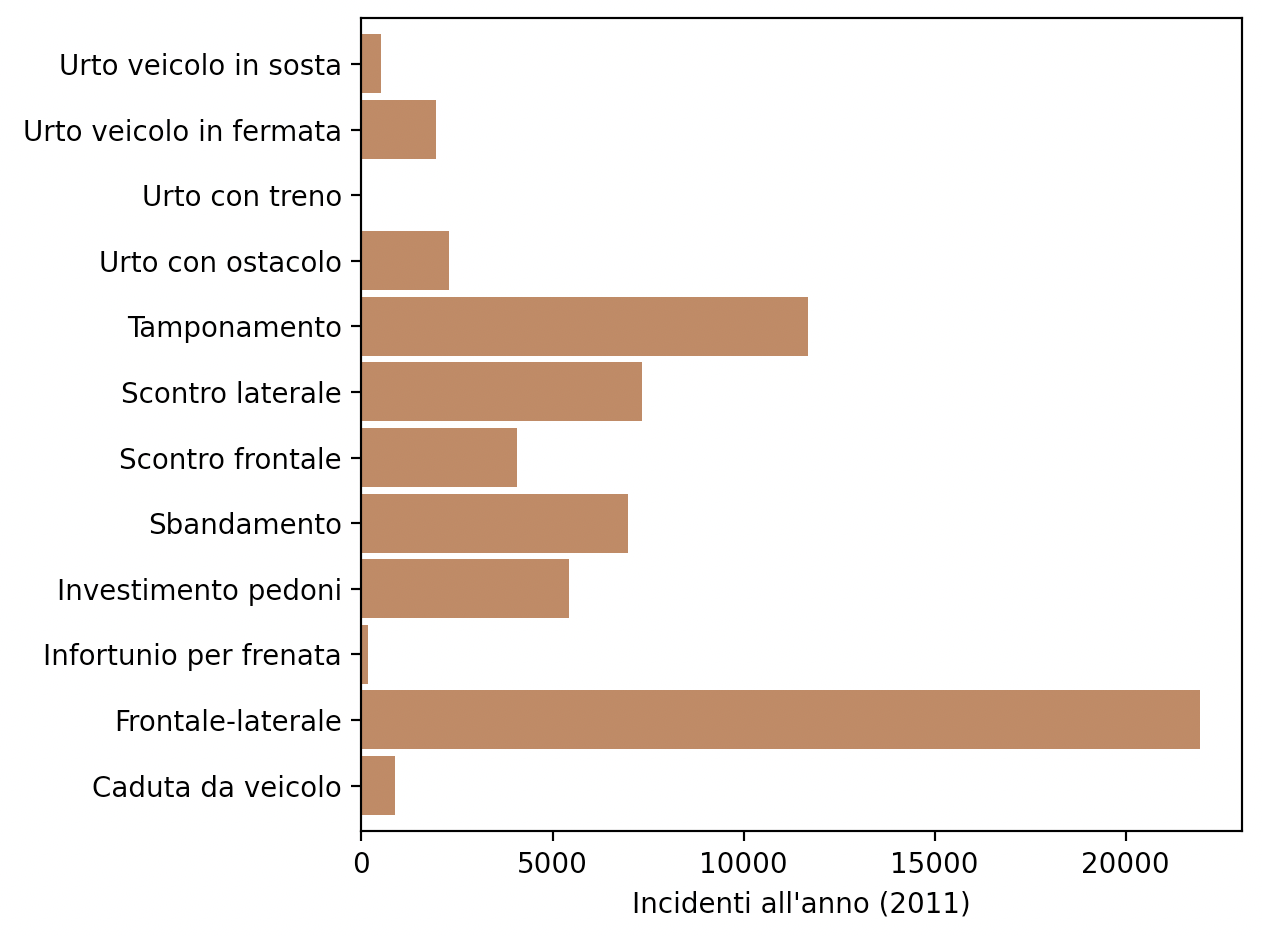
\includegraphics[width=\linewidth]{../src/incidenti/incidenti_senza_coords/localizzazione_incidente/tipo_incidente.png}
    \caption{Tipologia di incidente}
    \label{fig:tipo_incidente}
\end{figure}

Sono molto frequenti scontri frontali, laterali e tamponamenti.

%\clearpage
\subsection{Quali tipi di incroci provocano più incidenti?}

\begin{figure}
    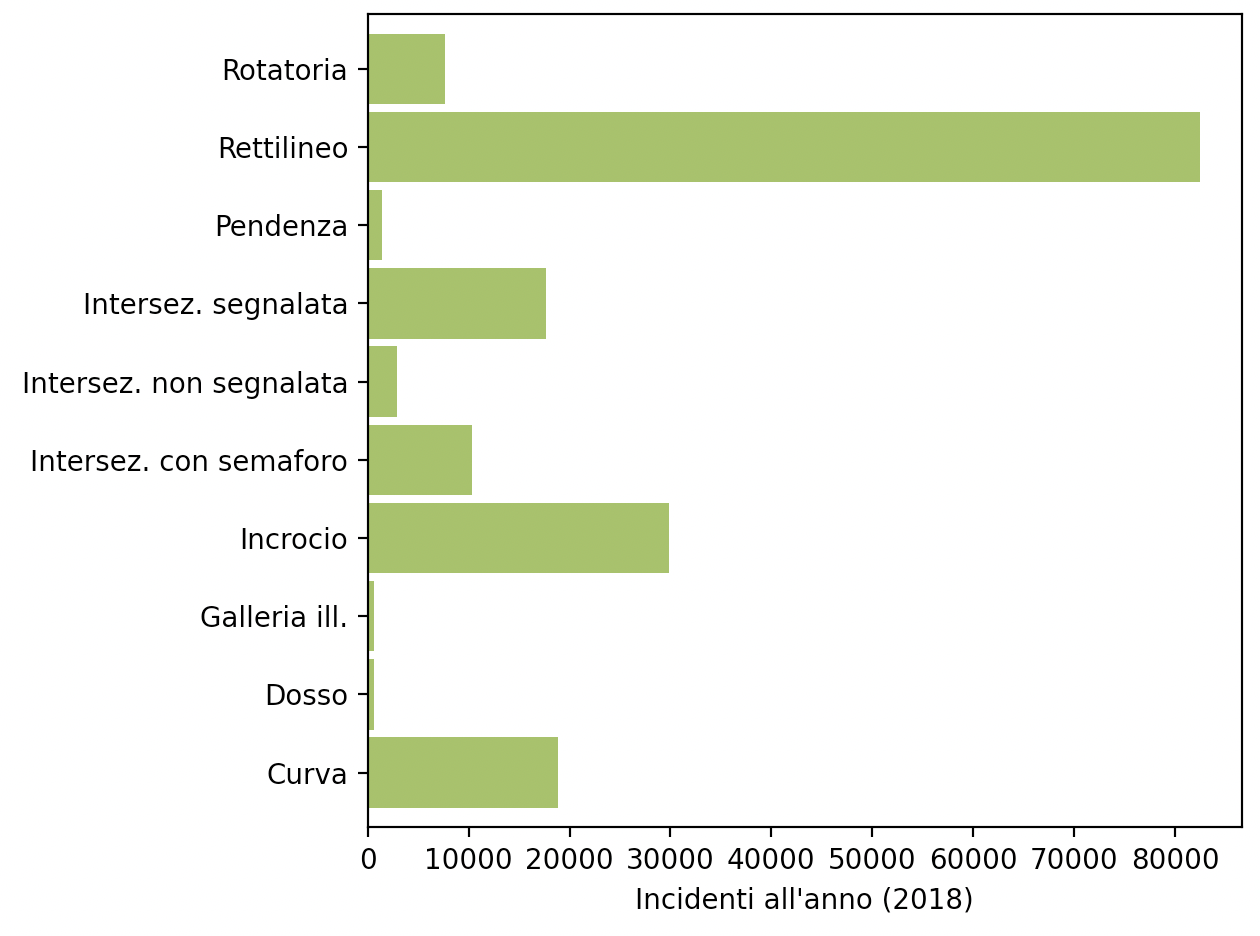
\includegraphics[width=\linewidth]{../src/incidenti/incidenti_senza_coords/localizzazione_incidente/intersezioni.png}
    \caption{Tipologia di intersezioni}
    \label{fig:tipo_intersezioni}
\end{figure}

La maggior parte degli incidenti avviene nei rettilinei e negli incroci.

%...

%\clearpage
\subsection{Esistono tipi di incidenti che provocano più feriti?}

\begin{figure}
    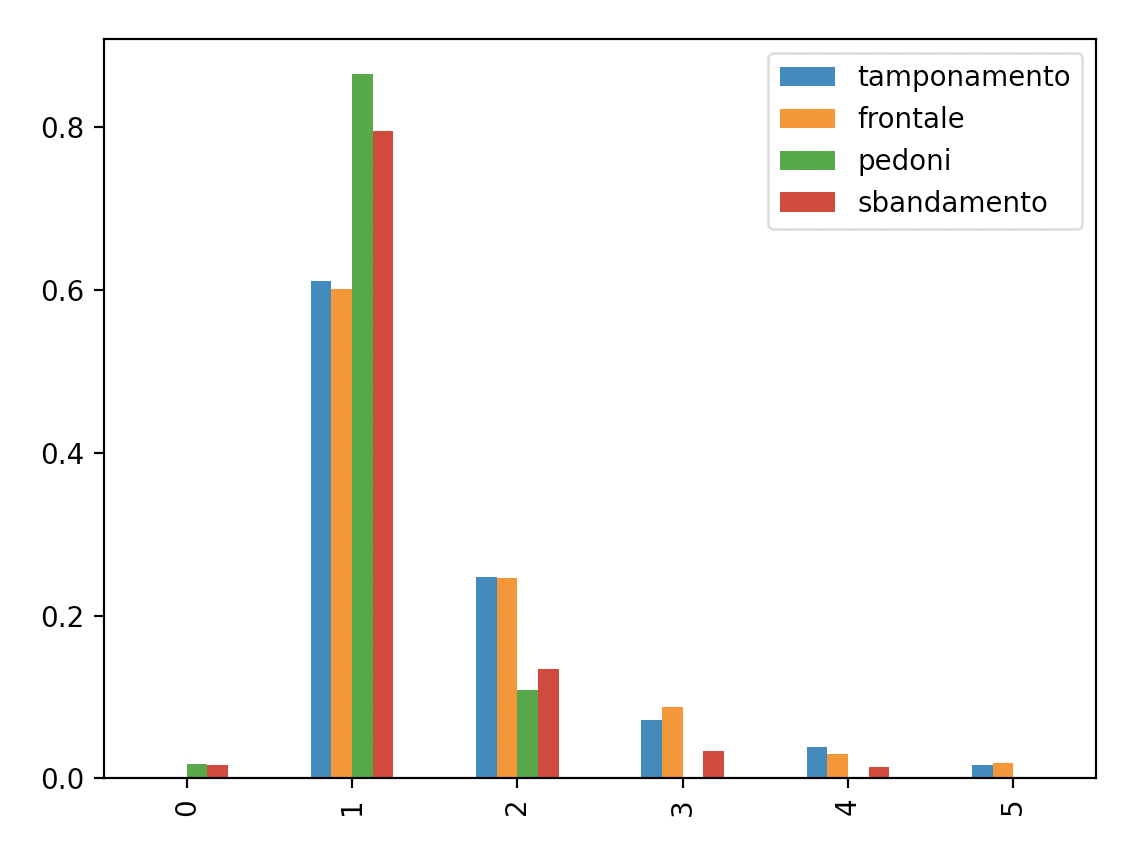
\includegraphics[width=\linewidth]{../src/incidenti/incidenti_senza_coords/natura_incidente/numero_feriti.png}
    \caption{Numero di feriti in base alla natura dell'incidente}
    \label{fig:numero_feriti}
\end{figure}

Si nota che esistono tipologie di sinistri che favoriscono la presenza di un solo ferito, 
come gli incidenti con pedone. Al contrario, incidenti come il tamponamento e frontale, 
hanno un'alta percentuale di situazioni con due o più feriti.


%\clearpage
\subsection{Esistono incroci che favoriscono incidenti con pedoni?}

\begin{figure}
    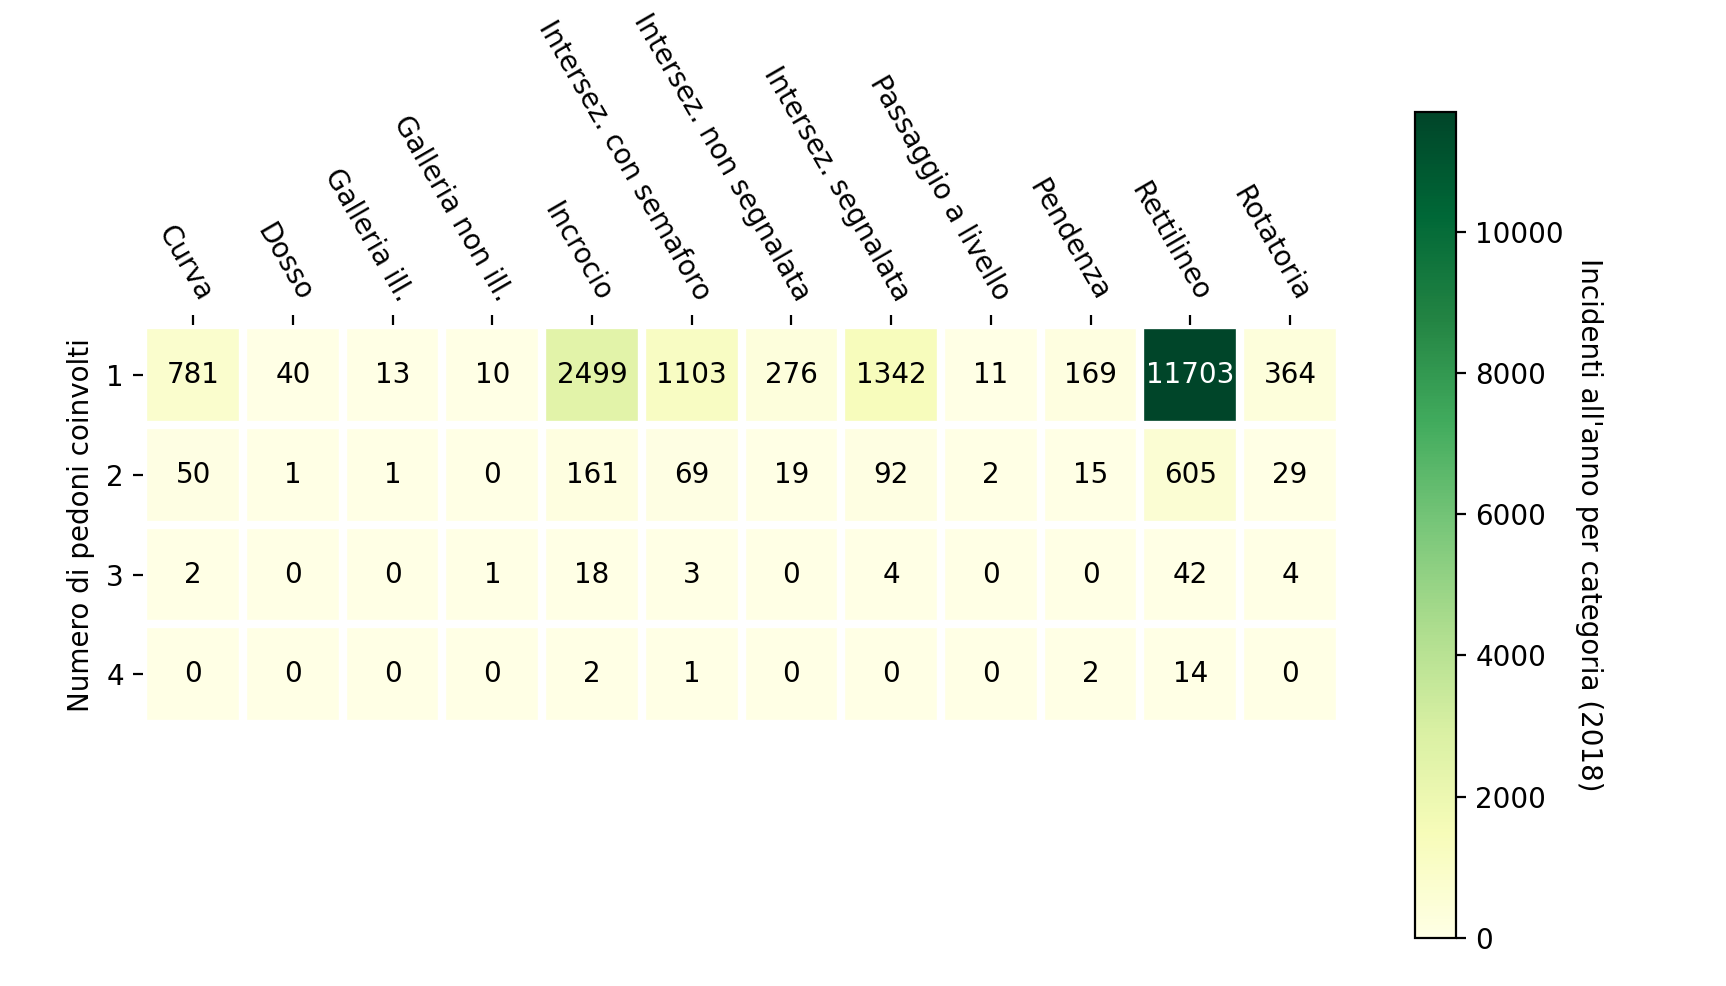
\includegraphics[width=\linewidth]{../src/incidenti/incidenti_senza_coords/pedoni/pedoni_incroci.png}
    \caption{Tipologia di intersezioni e pedoni coinvolti}
    \label{fig:pedoni_intersezioni}
\end{figure}

\todo{Trovare un modo per dividere pedoni\_feriti e tipo\_incrocio}
\begin{center}
    \def\arraystretch{1.5}%  
    \begin{tabular}{ |c|c|c|c|c| } 
    \hline
    pedoni\_feriti            &  1  & 2   & 3   & 4  \\
    tipo\_incrocio            &     &     &     &    \\
    \hline
    Curva                    & 195 &  15 &   1 &   0\\
    Dosso                    &  17 &   0 &   0 &   0\\
    Incrocio                 & 740 &  55 &   2 &   0\\
    Intersez. con semaforo   & 250 &  20 &   1 &   0\\
    Intersez. non segnalata  &  89 &   5 &   0 &   0\\
    Intersez. segnalata      & 335 &  19 &   2 &   1\\
    Passaggio a livello      &   1 &   0 &   0 &   0\\
    Pendenza                 &  42 &   4 &   1 &   1\\
    Rettilineo               &3369 & 206 &  18 &   6\\
    Rotatoria                & 134 &  10 &   0 &   0\\
    \hline
    \end{tabular}
\end{center}


Tra i tipi di strada che favoriscono incidenti con pedoni spiccano i rettilinei, 
probabilmente in parte per l'alta velocit\'a dei veicoli, ma anche per l'alto volume di
tratti di strada di questo tipo.

%...

%\clearpage
\subsection{Ci sono aspetti salienti sui pedoni coinvolti?}

\begin{figure}
    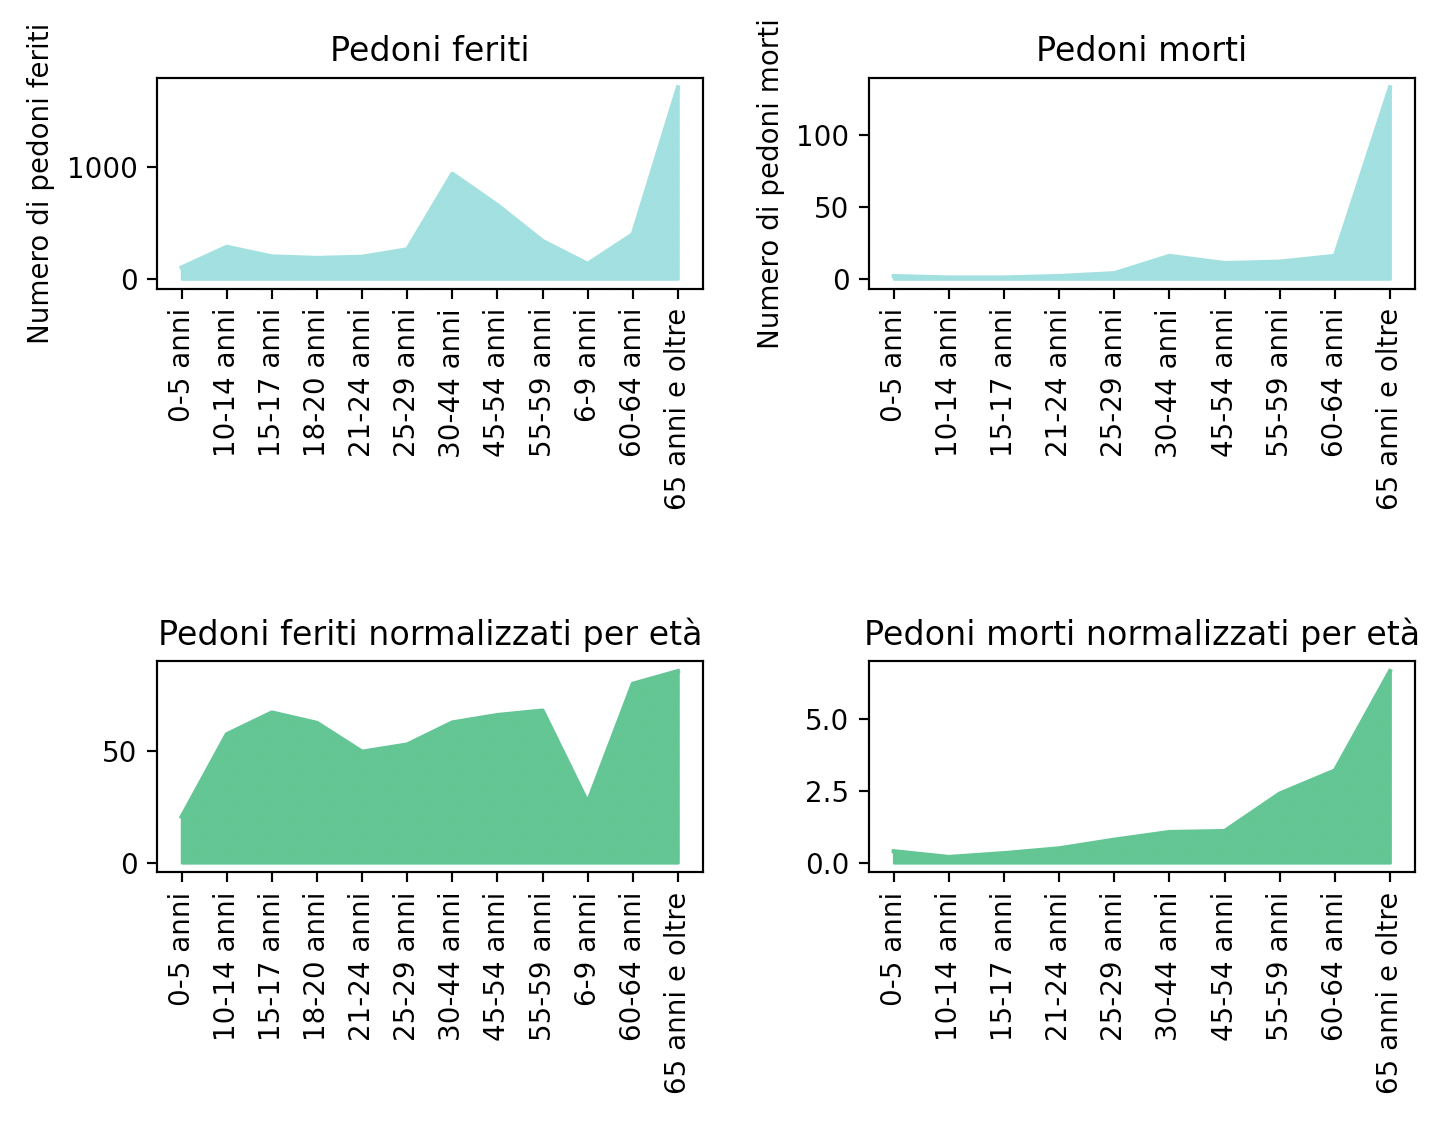
\includegraphics[width=\linewidth]{../src/incidenti/incidenti_senza_coords/pedoni/eta_pedoni.png}
    \caption{Fasce di et\'a dei pedoni coinvolti in incidenti}
    \label{fig:eta_pedoni}
\end{figure}

La fascia di et\'a più colpita dagli incidenti è quella dei 65 anni, 
va comunque detto che questo gruppo probabilmente contiene la maggior parte degli individui.
Se si normalizza per anni contenuti in ogni fascia, ipotizzando un numero
costante di persone di ogni et\'a, si ottiene un grafo, per quanto riguarda i pedoni 
feriti, molto differente. \\
La normalizzazione tiene conto che la fascia di et\'a '65 anni e oltre' vale venti anni.
%...

\begin{figure}
    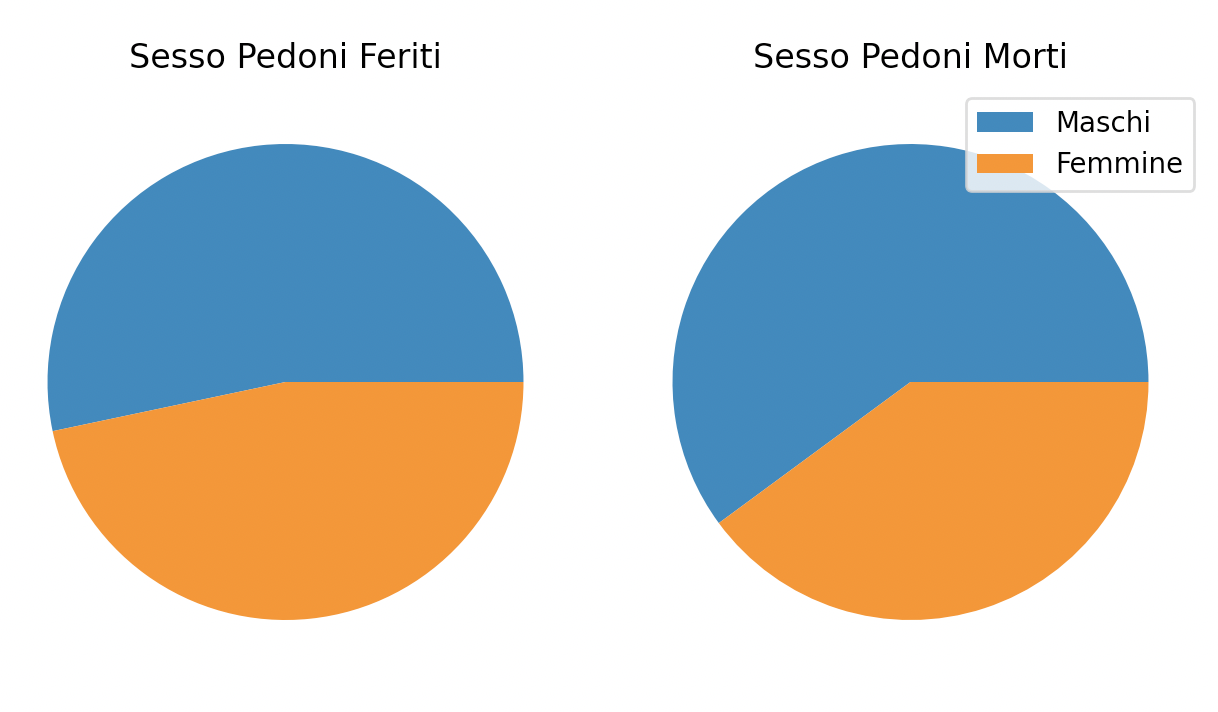
\includegraphics[width=\linewidth]{../src/incidenti/incidenti_senza_coords/pedoni/sesso_morti_feriti.png}
    \caption{Pedoni coinvolti in incidenti per genere}
    \label{fig:sesso_morti_feriti}
\end{figure}

Dati non sorprendenti\dots

%...




%\clearpage
\section{Dati ACI}

%\clearpage
\subsection{Esiste correlazione tra incidenti e feriti?}

E allo stesso modo, esiste correlazione tra morti e incidenti, o tra morti e feriti?\\
Ovviamente si attende un esito positivo a queste domande.
L'indice di correlazione utilizzato è il coefficiente di Pearson.
%TODO: formula?
\begin{center}
    \begin{tabular}{ |c|c|c| } 
    \hline
    Incidenti & Incidenti & Feriti \\ 
    Feriti & Morti & Morti \\ 
    \hline
    0.9827 & 0.8205 & 0.8332 \\ 
    \hline
    \end{tabular}
\end{center}

Il coefficiente di Pearson, per quanto riguarda Incidenti e Feriti, 
è molto vicino a uno, quindi i due campioni sono strettamente correlati.
I coefficienti riguardanti i morti sono meno vicini uno, probabilmente per il minor numero 
di incidenti mortali, che rendono il campione più ristretto

\begin{figure}
    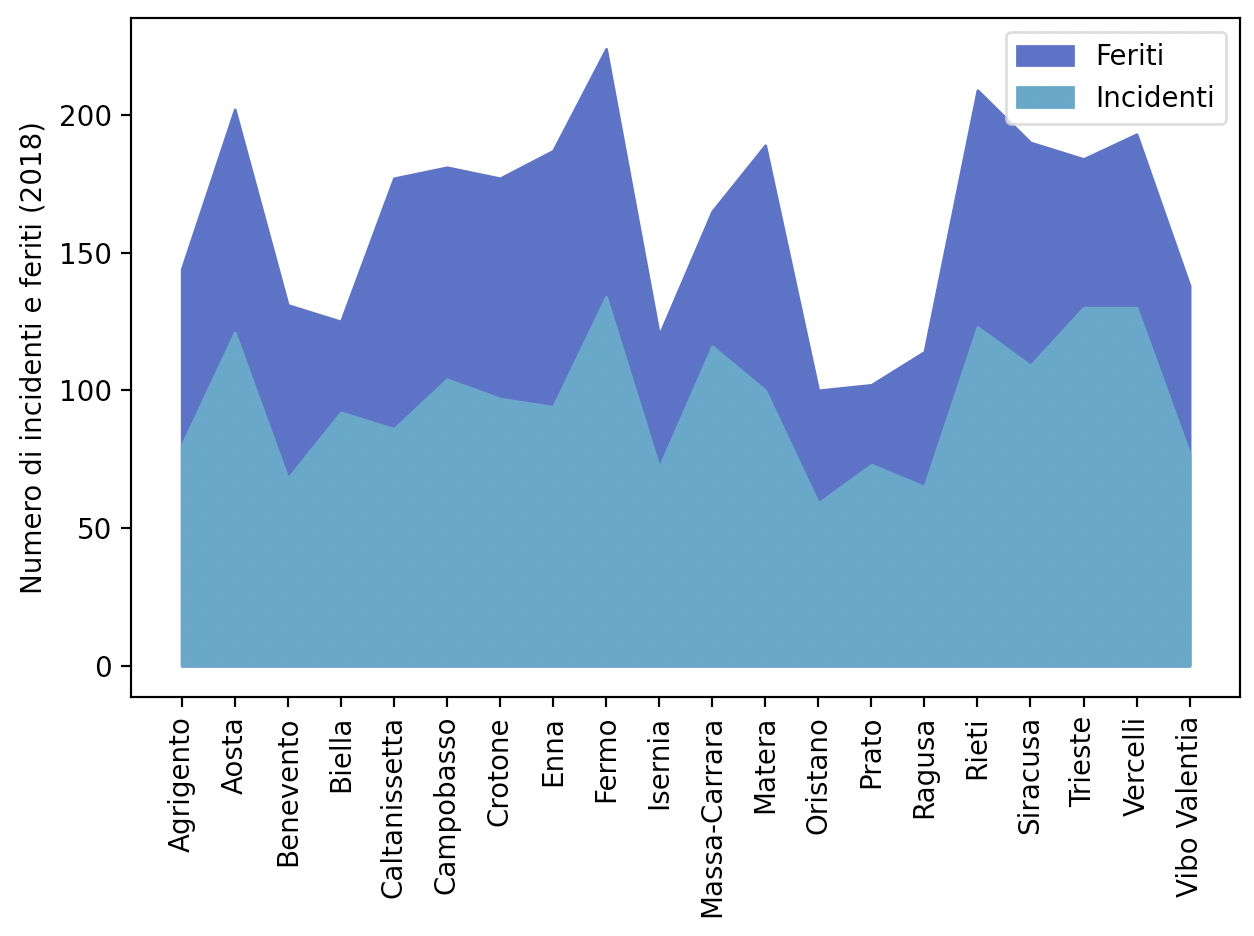
\includegraphics[width=\linewidth]{../src/incidenti/incidenti_aci/comuni/corr_incidenti_feriti.png}
    \caption{Correlazione tra numero di feriti e incidenti}
    \label{fig:corr_incidenti_feriti}
\end{figure}

Tracciando il grafo dei primi trenta valori del dataset ACI, 
è chiaramente visibile la correlazione tra numero di incidenti e numero di feriti.



%\clearpage
\subsection{Quali sono le autostrade con più incidenti?}
\begin{figure}
    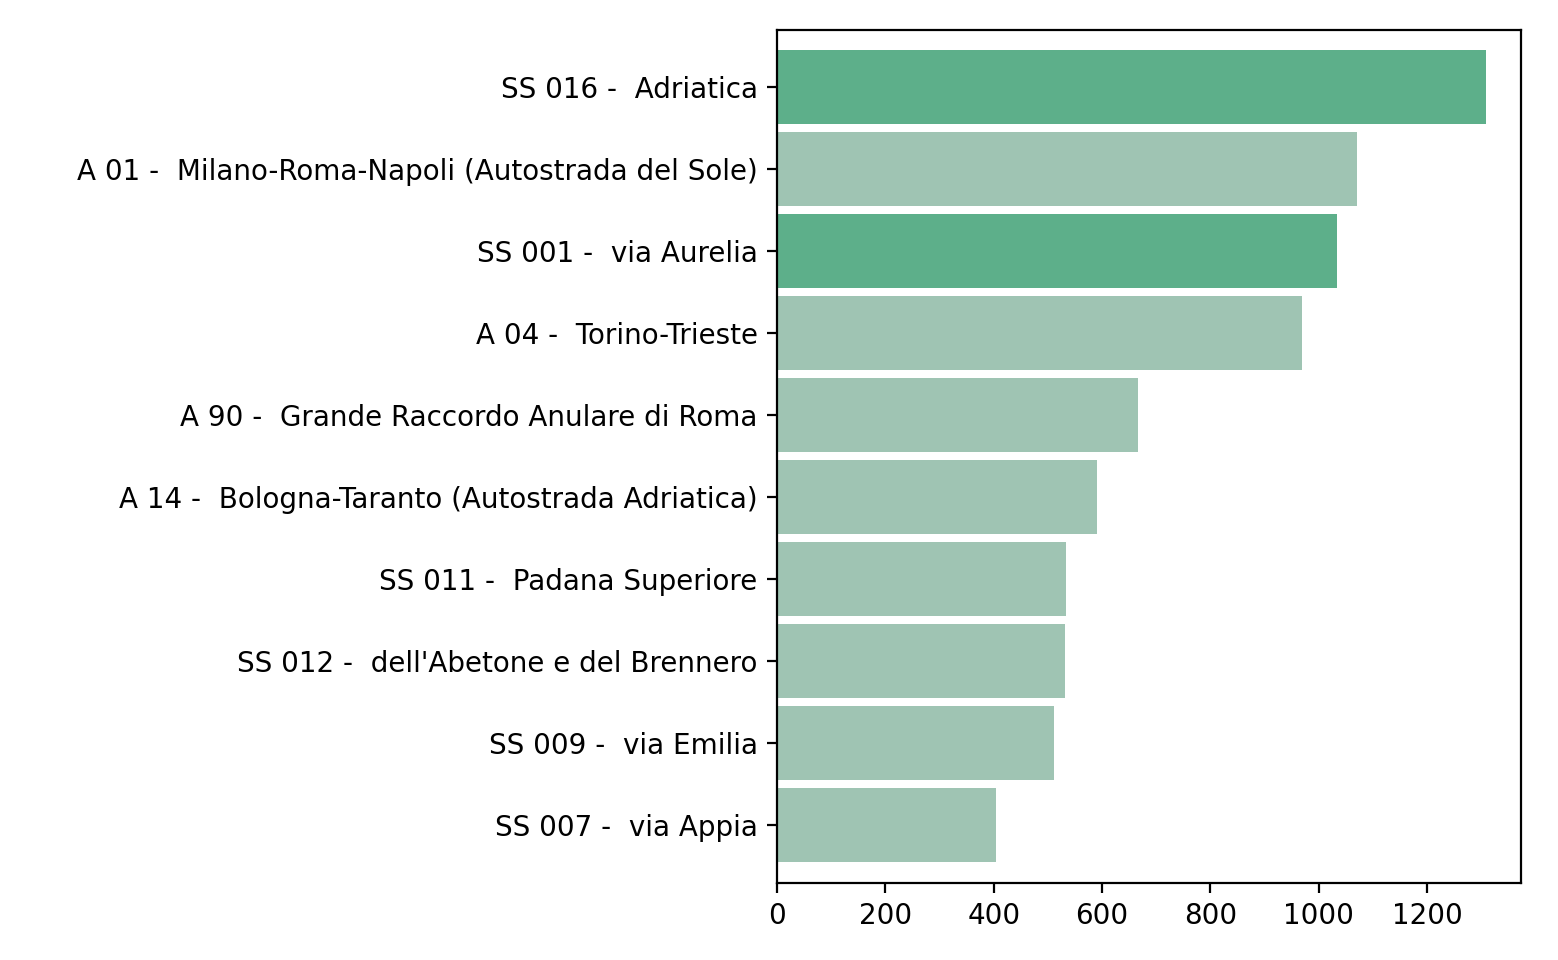
\includegraphics[width=\linewidth]{../src/incidenti/incidenti_aci/autostrade/autostrade.png}
    \caption{Autostrade con più incidenti nel 2018}
    \label{fig:incidenti_autostrade}
\end{figure}

Si pu\'o notare subito che le autostrade con più incidenti sono anche quelle più trafficate, come 
l'Autostrada del Sole e l'Adriatica.


%...


%\clearpage
\subsection{Autostrade pericolose a Milano?}

\begin{figure}
    \includegraphics[width=\linewidth]{../src/incidenti/incidenti_aci/autostrade/incidenti_bubble_chart.png}
    \caption{Autostrade con più incidenti nel 2012}
    \label{fig:bubble_incidenti_milano}
\end{figure}



%...

%\clearpage
\subsection{In quali mesi avvengono più incidenti?}
\begin{figure}
    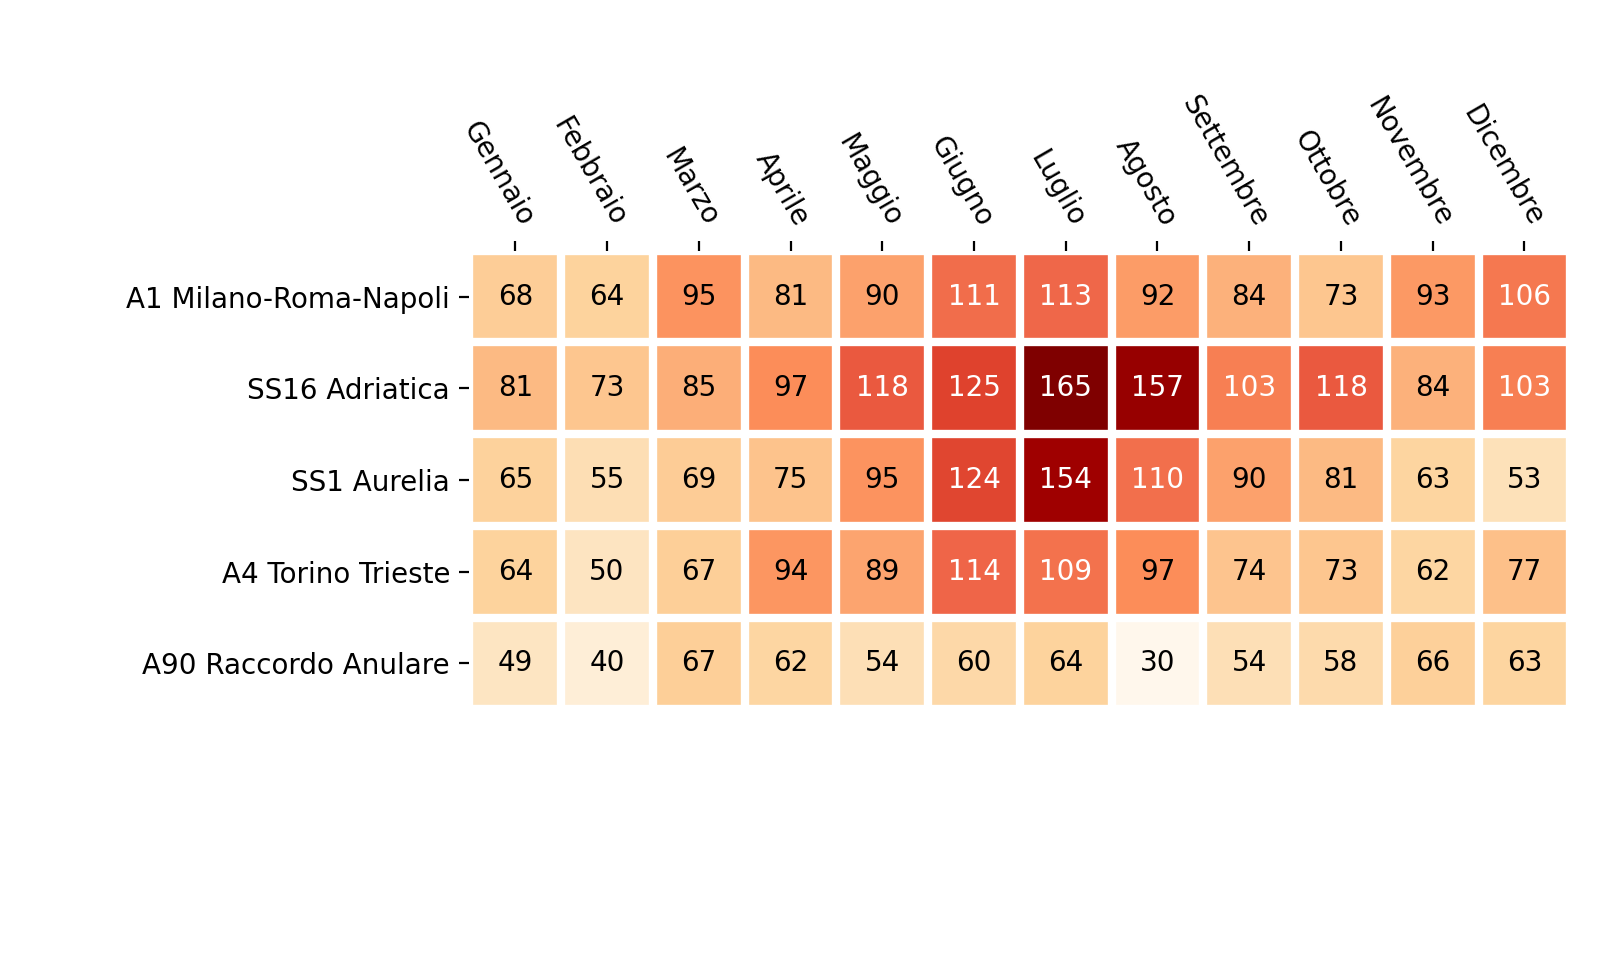
\includegraphics[width=\linewidth]{../src/incidenti/incidenti_aci/autostrade/mesi_autostrade.png}
    \caption{Incidenti per mese nel 2018}
    \label{fig:incidenti_per_mese}
\end{figure}

Le curve sono state normalizzate per bilanciare il volume di incidenti maggiori per 
l'autostrada Adriatica.
L'Adriatica e l'Aurelia, autostrade utilizzate molto durante i mesi caldi, hanno un picco di 
incidenti in Luglio e Agosto, mentre l'A1, ha picco più basso in Agosto, probabilmente 
perchè bilanciato dagli incidenti in inverno intorno a Milano.

% controllare se avvengono più incidenti in inverno intorno a milano
Infatti se si prendono solo i dati della A1 nella provincia di Milano, si nota 
che in Maggio e Settembre avvengono la maggior parte degli incidenti.
Invece sull'Adriatica prevalgono incidenti in Luglio e Agosto.
\begin{figure}
    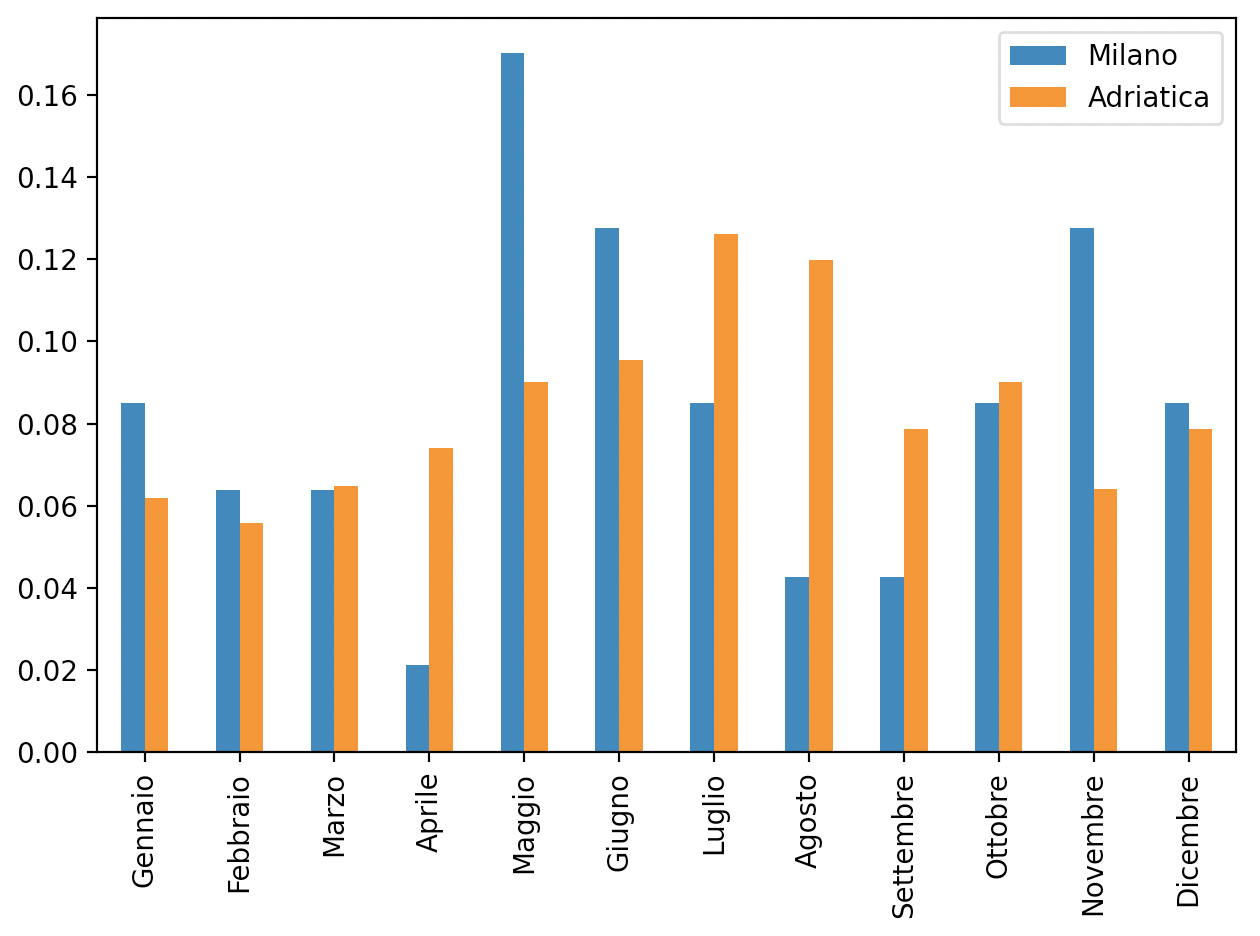
\includegraphics[width=\linewidth]{../src/incidenti/incidenti_aci/autostrade/milano_adriatica.png}
    \caption{Incidenti in provincia di Milano e sull'Adriatica}
    \label{fig:milano_adriatica}
\end{figure}

%...

%\clearpage%
\subsection{In Quali orari avvengono incidenti sulle autostrade?}
\todo{orari di altri luoghi, ho fatto solo milano}

\begin{figure}
    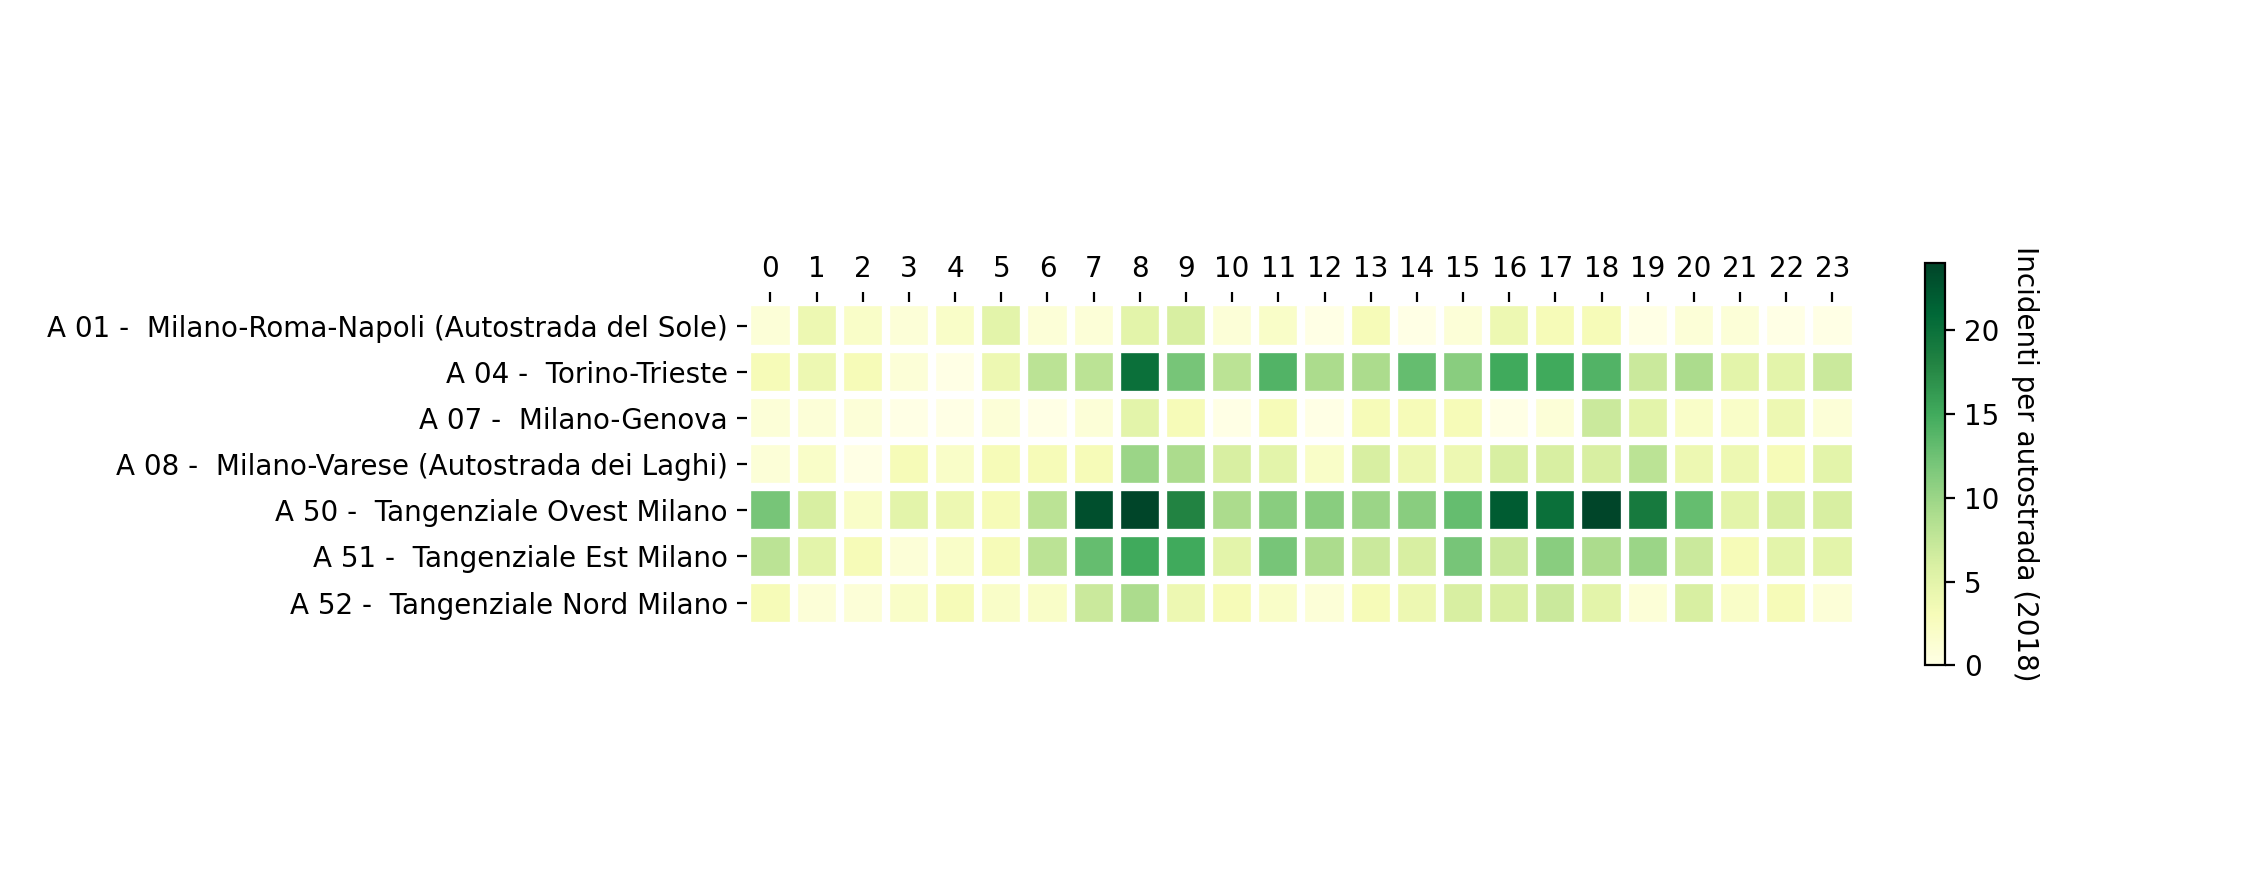
\includegraphics[width=\linewidth]{../src/incidenti/incidenti_aci/autostrade/tangenziali_autostrade.png}
    \caption{Incidenti nelle principali autostrade di Milano}
    \label{fig:tangenziali_autostrade}
\end{figure}

\begin{figure}
    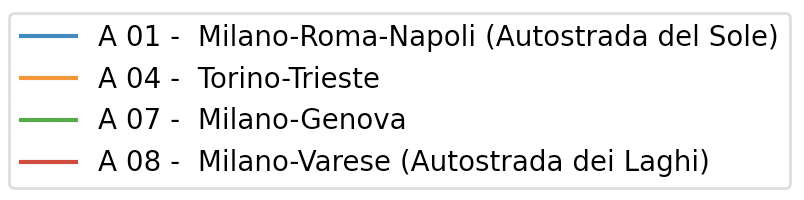
\includegraphics[width=0.6\linewidth]{../src/incidenti/incidenti_aci/autostrade/legenda_autostrade.png}
    \label{fig:legenda_autostrade}
    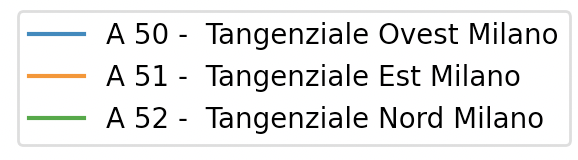
\includegraphics[width=0.5\linewidth]{../src/incidenti/incidenti_aci/autostrade/legenda_tangenziali.png}
    \label{fig:legenda_tangenziali}
\end{figure}

Il grafo conferma per alcune autostrade i picchi di incidenti per il traffico durante orari 
di punta, in particolare è molto visibile per la Torino$-$Trieste e per la Tangenziale ovest.

%...

%\clearpage
\subsection{Quali autostrade sono utilizzate di più per viaggiare in Agosto?}

\begin{figure}
    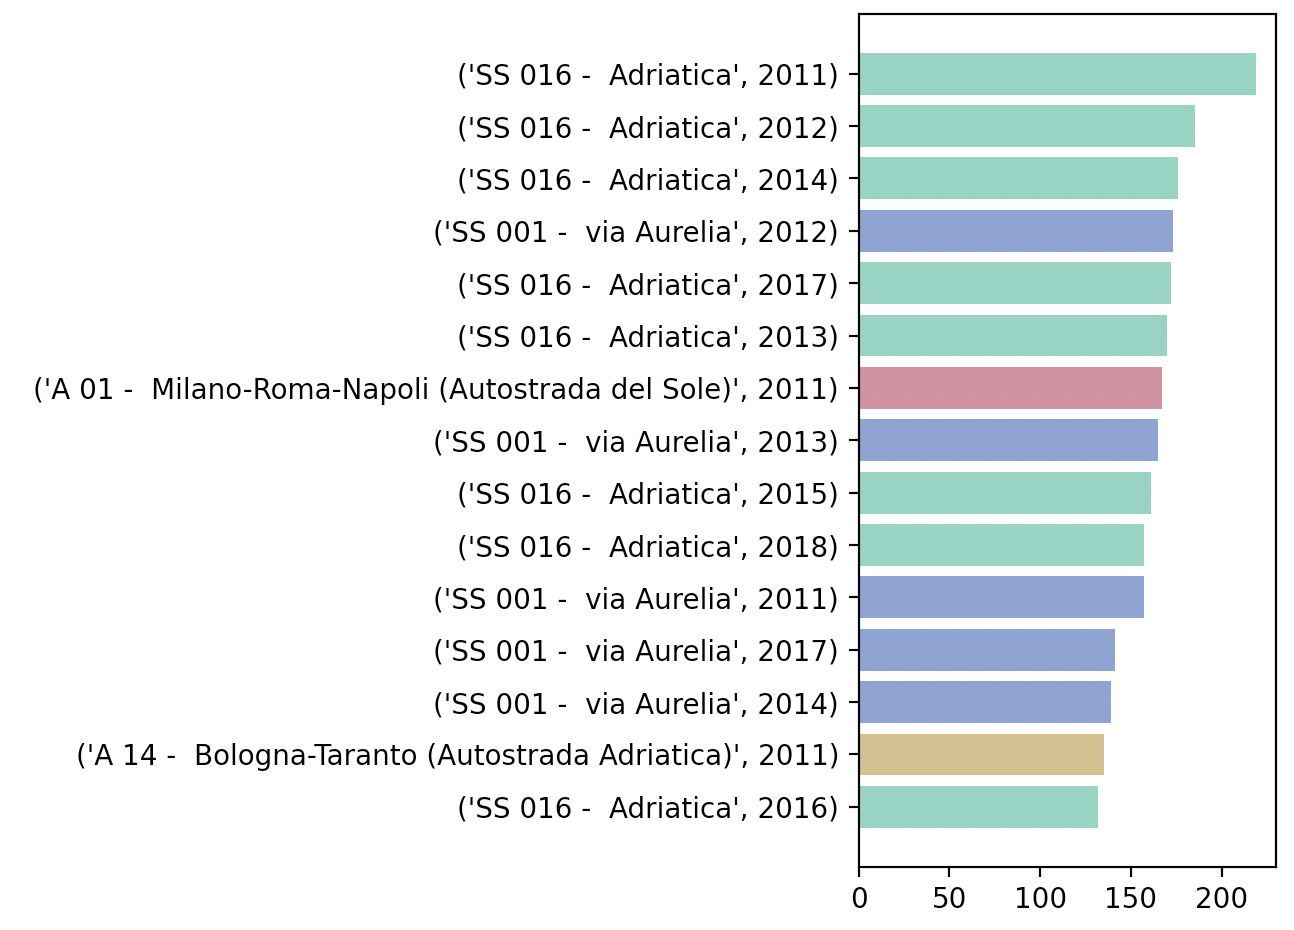
\includegraphics[width=\linewidth]{../src/incidenti/incidenti_aci/agosto/autostrade_anno_agosto.png}
    \caption{Autostrade con più incidenti per anno, in Agosto}
    \label{fig:autostrade_anno_agosto}
\end{figure}

Il grafo rappresenta in quali autostrade sono avvenuti più incidenti in base al mese di Agosto
del rispettivo anno.
Non è sorprendente che le autostrade caratterizzate da un alto numero di bollini rossi e neri 
siano anche le più pericolose.
In particolare spiccano la SS16 Adriatica e SS1 Aurelia, non è difficile trovare il motivo dell'alto numero di incidenti, 
queste ultime infatti sono Strade Statali molto lunghe e con corsie di marcia non separate, 
per non parlare del fatto che entrambe le strade passano attraverso un alto numero di centri abitati, 

\begin{figure}
    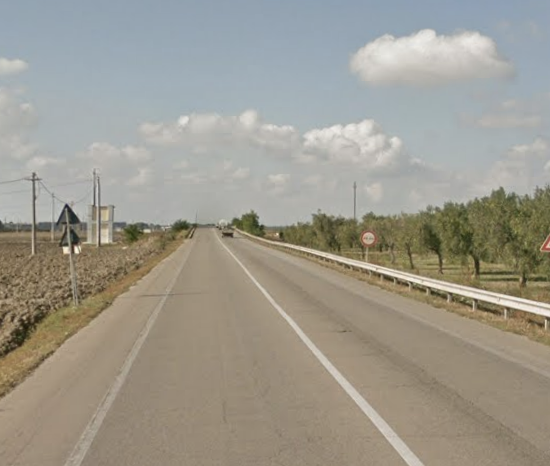
\includegraphics[width=\linewidth]{../src/incidenti/incidenti_aci/agosto/adriatica.png}
    \caption{SS16 Adriatica vicino Foggia}
    \label{fig:adriatica}
\end{figure}

%\clearpage
\subsection{Le autostrade più utilizzate cambiano a seconda dell'anno?}

Il numero di persone in vacanza nelle localit\'a del centro e sud italia cambiano 
a seconda dell'anno, il numero di incidenti rispecchia questo cambiamento?

\begin{figure}
    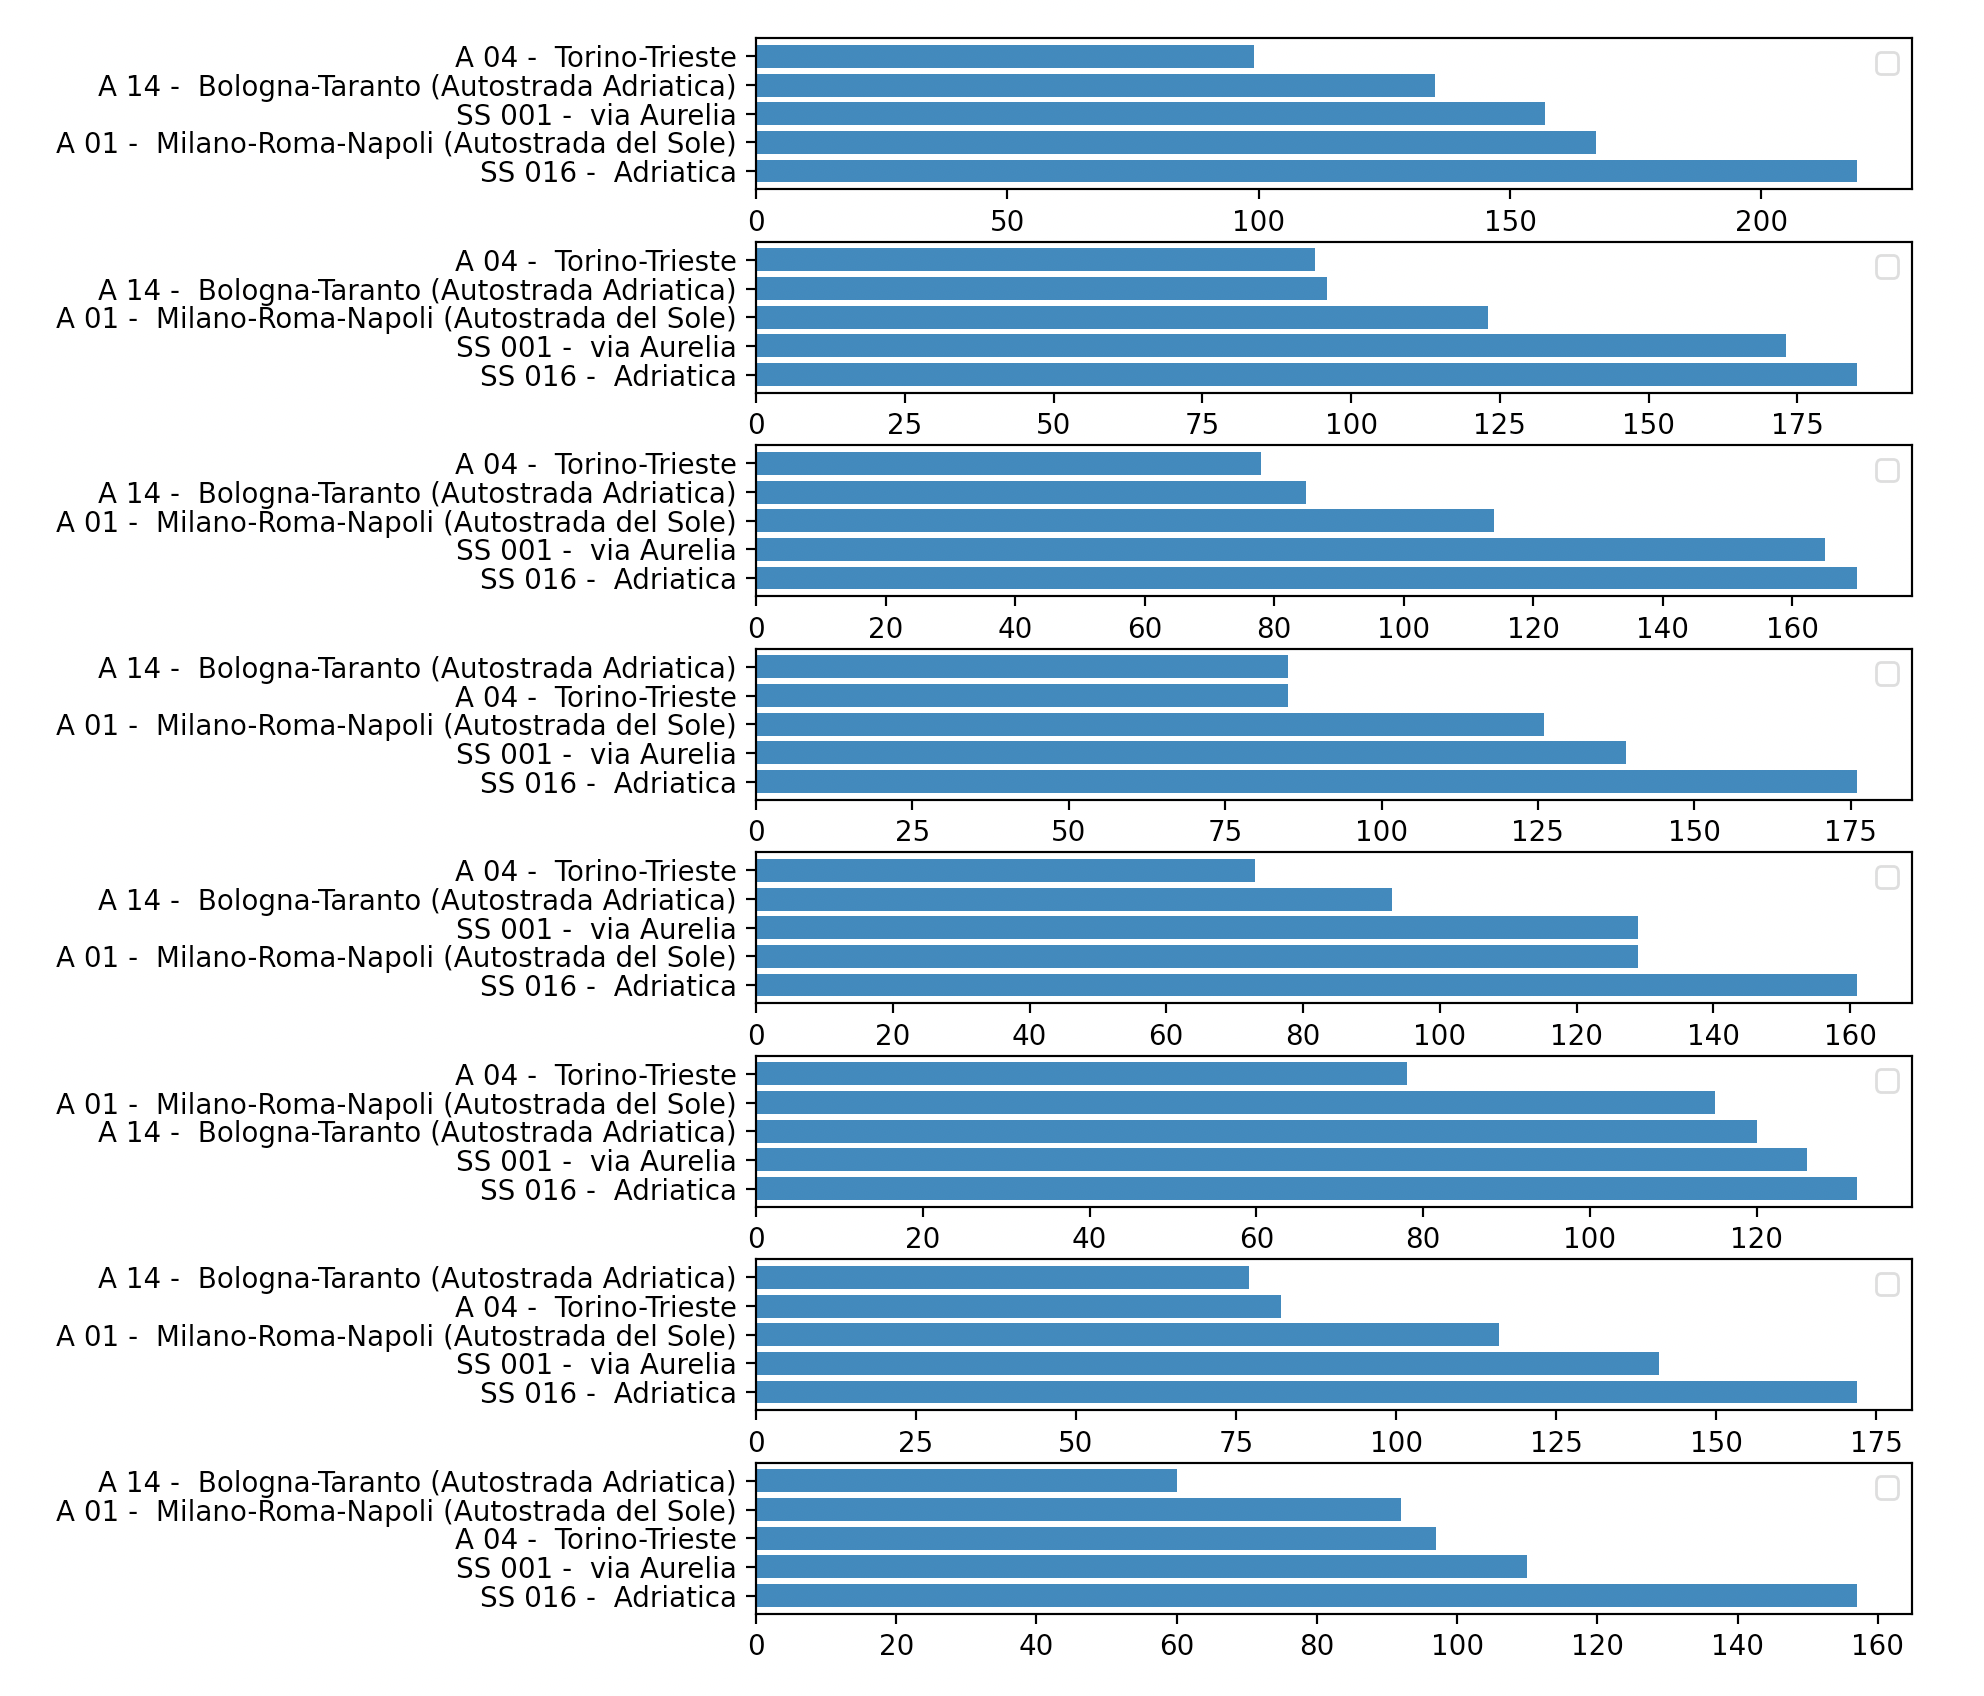
\includegraphics[width=\linewidth]{../src/incidenti/incidenti_aci/agosto/autostrade.png}
    \caption{Incidenti in Strade per anno}
    \label{fig:autostrade_anno}
\end{figure}

Controllando le prime cinque strade per incidentalit\'a ogni anno, si ottiene un'immagine 
abbastanza stabile, in quanto gli itinerari in testa alla classifica sono sempre gli stessi.
Si nota, che la strada statale Adriatica è sempre in prima posizione, 
con una media di $171.5$ incidenti nel mese di Agosto.
Le posizioni successive invece cambiano a seconda dell'anno, in particolare per\'o, l'autostrada 
A4 (Torino-Trieste) ha progressivamente aumentato il numero di incidenti, evento possibilmente 
dovuto all'aumento di popolarit\'a delle vacanze in montagna.
% Posso provarlo con dati istat a
% https://www.istat.it/it/archivio/178695


%%%%%%%%%%%%%%%%%%%%%%%%%%%%%%%%%%%%%%%%%%%%%%%%%%%%%%
%\clearpage
\chapter{Dati su Meteo}

\bibliographystyle{plain}
\bibliography{Biblio}
%\addcontentsline{toc}{chapter}{Bibliografia}

\end{document}
